\documentclass{article}
\usepackage{graphicx}
\usepackage[margin=1.4in]{geometry}
\usepackage{booktabs}
\usepackage{subfigure}
\usepackage{placeins}

\begin{document}

\title{Udacity ML Engineer Nanodegree \\ Capstone Project \\ Acea Smart Water Analysis}
\author{Rose Koopman}
\date{}
\maketitle


\section{Definition}

\subsection*{Project Overview}

In the last decade humanity faced unprecedented challenges due to rising sea water level, flooding of rivers, draughts and overall more extreme whether conditions. With the effects of climate change becoming a severe thread to humanity, the monitoring of water supplies becomes of increasing importance. 

With a service area covering over 9 million people, the Acea Group \cite{acea} is one of Italy's leading companies in the field of water supply. Its main responsibilities include building and maintaining a water network and preserving the health of its water bodies,  in order to guarantee the daily water supply to Italy's inhabitants. 

The Acea Groups utilises different types of water bodies:

\begin{itemize}
\item Aquifer: A water-containing layer (such as sand) in the ground. Water can be taken from the aquifer by making a well. 
\item Water spring: The place where an underground water body (e.g. underground river) emerges at the earth's surface.
\item River: A flowing body of water, typically flowing from a water spring to the ocean.
\item Lake: A contained body of water which is surrounded by land. There can be a river feeding into the lake and another river draining the lake.
\end{itemize}


\subsection*{Problem Statement}

In order to provide in the daily water consumption, Acea Group carefully monitors the water level and water flow in its different water bodies. Each of these types of water bodies have their own characteristics and respond in a different way to events of rainfall or periods with high temperatures. Typically water bodies fill in autumn and winter when more water enters the bodies then is being utilised, while in spring and autumn water levels drop. In order to guarantee continuous water supply and preserve the health of the water bodies, there is a need to forecast water availability in terms of level and flow.

The task at hand it to build a predictive model which predicts either water level or water flow for several water bodies.\footnote{This problem is published as a Kaggle competition~\cite{kaggle}} Since the type of features and target depend on the type of water body, a different model needs to be made for each type of water body. As the differences between water bodies of the same type can be large, and the availability of features differs, it might be necessary to create a separate model for each individual water body. 

%prediction horizon!

\subsection*{Metrics}

Model evaluation will be done by $R^2$, in order to provide a measurement of the amount of variance captured by the features. In order to get a feel for the size of the errors, additionally the $RMSE$ and $MAE$ will be used. A comparison between the values of $RMSE$ and $MAE$ can tell something about the type of errors the model makes: many small errors or a few large errors. 

In order to compare models of the same type applied to different datasets the $MAPE$ will be used. As this concerns a relative error, results on different datasets where target values can be different in orders of magnitude can be compared. This way it might be possible to find the type of model which works best for all water bodies (of one type), and have a more uniform approach across all water bodies to forecast water level and flow.


\section{Analysis}

\subsection*{Data Exploration}

The Acea Groups utilises different types of water bodies. Data is provided for four aquifers, three water springs, one river and one lake. As can be seen in Fig.~\ref{fig:prep_ntargets} the number of available features differs greatly per water body. It should also be noted that multiple targets can be available for one water body, corresponding to different geographically located measurement points. Depending on the type of water body, different measurements are available as shown in Table~\ref{tab:targets_features}. The available measurements are:

\begin{itemize}
\item Depth to Groundwater ($m$): groundwater level measured using a piezometer
\item Flow Rate ($L/s$ or $m^3/s$)): flow rate of spring ($L/s$) or river ($m^3/s$) 
\item Hydrometry aquifer ($m$): groundwater level measured using the hydrometric station
\item Hydrometry river ($m$): river level measured using the hydrometric station
\item Lake Level ($m$): river level
\item Volume ($m^3$): volume of water taken from the drink water treatment plant
\item Rainfall ($mm$): quantity of rain fall
\item Temperature ($^{\circ}C$): temperature
\end{itemize}

As an example, a data extract is provided in Table~\ref{tab:sample}. 

Although the datasets span over several years and many features are provided for most water bodies, there are many periods where either one or multiple measurements are missing (see Fig.~\ref{fig:prep_nan}). Selecting only records where all measurements are available reduces the amount of available data with on average $60\%$ (ranging from $7\%$ to $97\%$ depending on the water body) making a large proportion unsuitable for modelling. As data unavailability is not sporadic, but rather seems to occur in large periods in time imputation of missing values by interpolation is impossible. The data collection period for both targets and features for one water body does often not align, and there can be periods in which data collection has been temporarily discontinued, as shown in Figure~\ref{fig:prep_missing_data}.

Due to the (un)availability of data the following water bodies are selected for a proof of concept:
 \begin{itemize}
	\item Aquifer Auser
	\item Aquifer Petrignano
	\item River Arno
	\item Lake Bilancio
\end{itemize}
Based on the learnings drawn from modelling these water bodies, advise can be given on the data collection of the other water bodies.


\begin{figure}[p]
\begin{center}
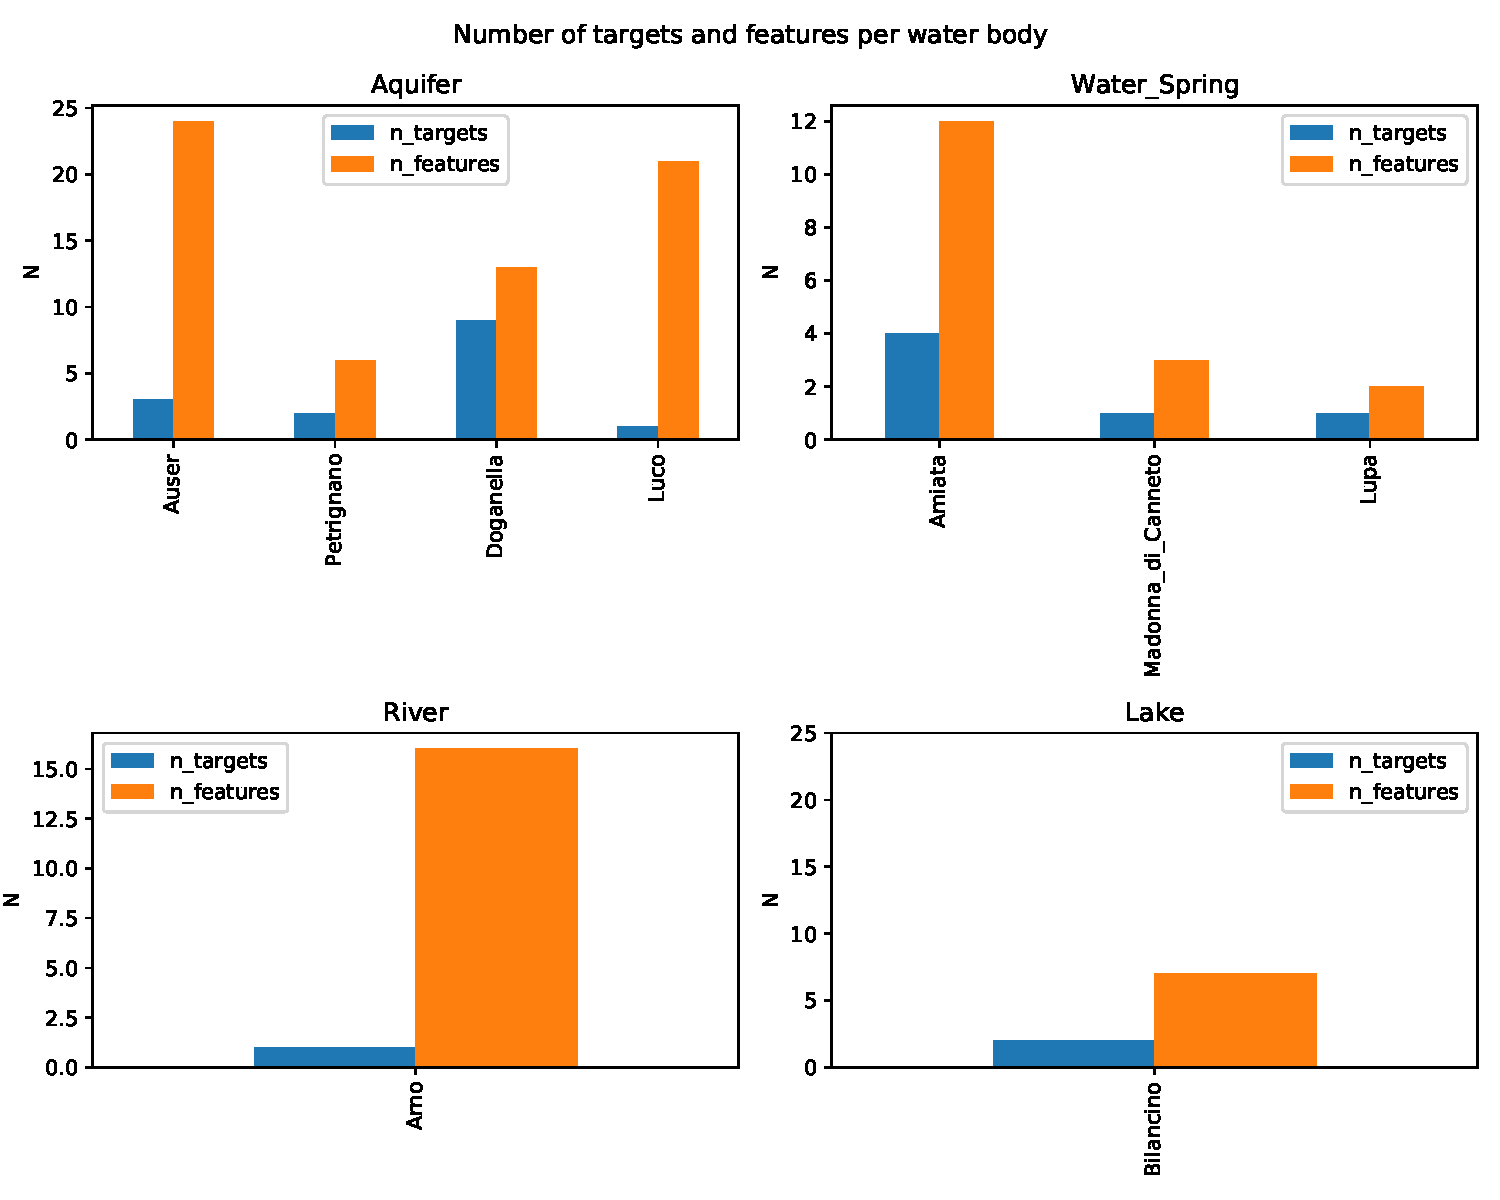
\includegraphics[width=0.9\textwidth]{figs/Number_of_targets_and_features_per_water_body.pdf}
\caption{The number of targets and features differs greatly between the different (types of) water bodies.}
\label{fig:prep_ntargets}
\end{center}
\end{figure}

\begin{figure}[p]
\begin{center}
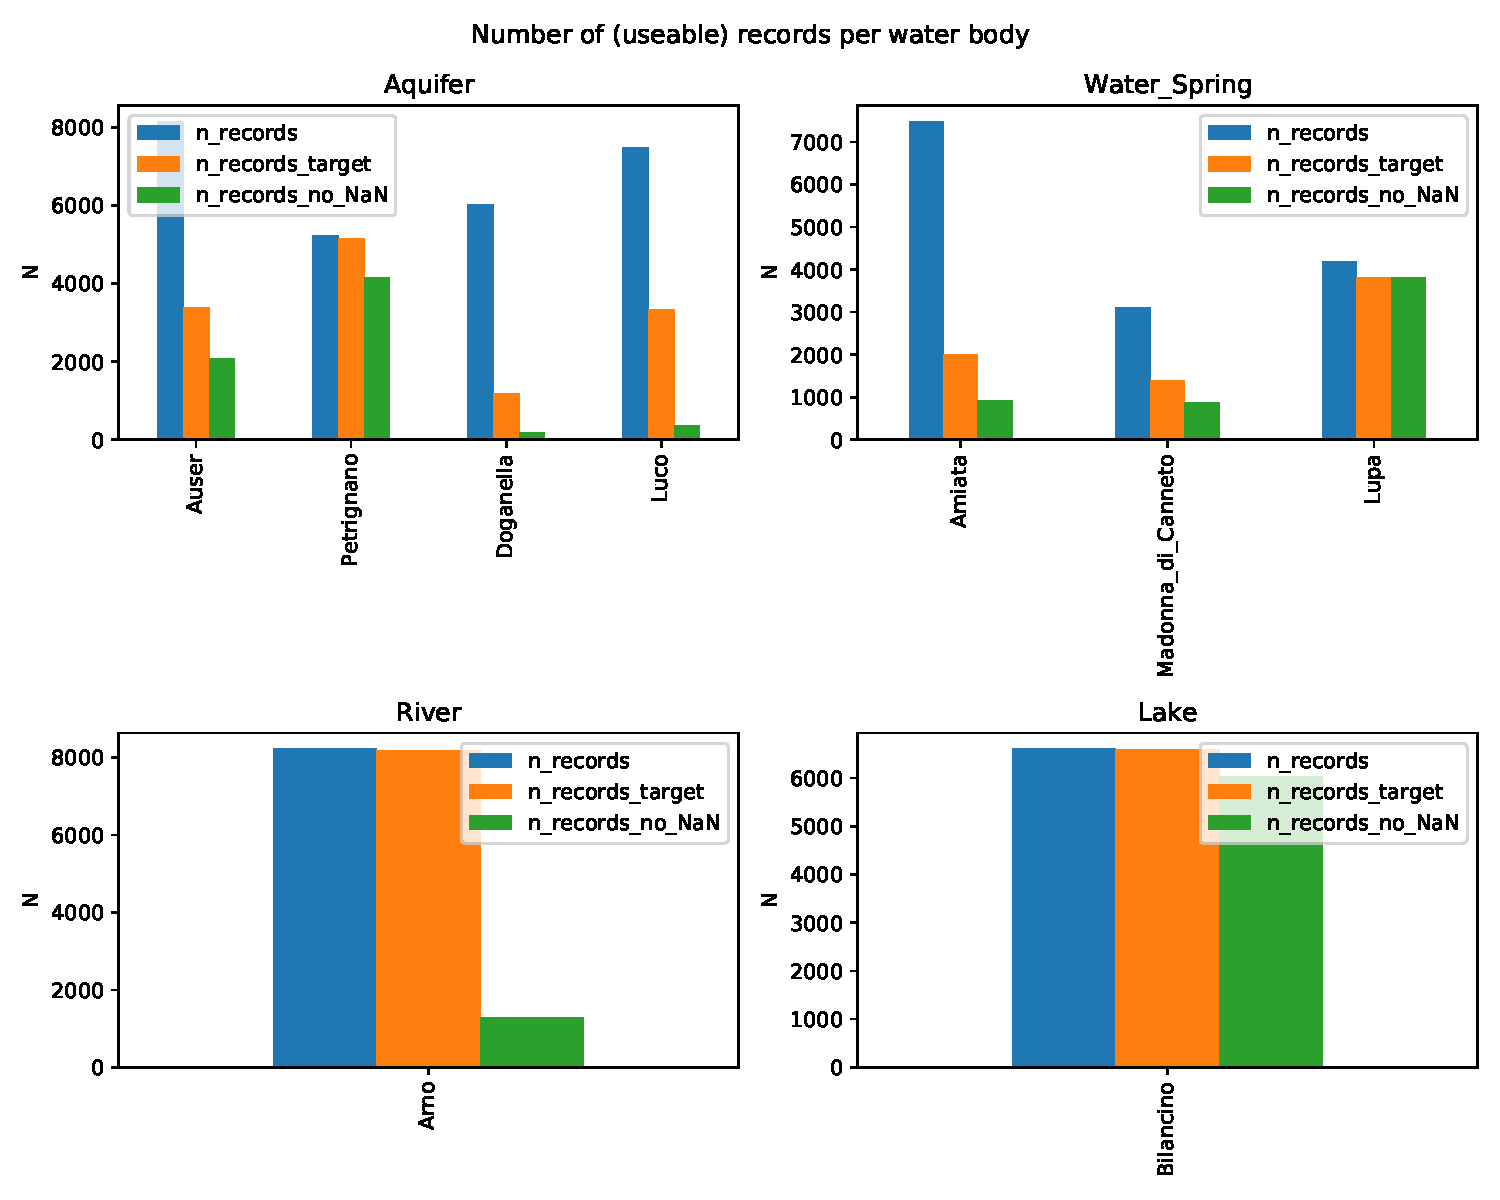
\includegraphics[width=0.9\textwidth]{figs/Number_of_(useable)_records_per_water_body.pdf}
\caption{Many measurements are unavailable for long periods of time. This concerns both measurements related to the target variables and measurements related to features. }
\label{fig:prep_nan}
\end{center}
\end{figure}

\begin{figure}[htb]
\begin{center}
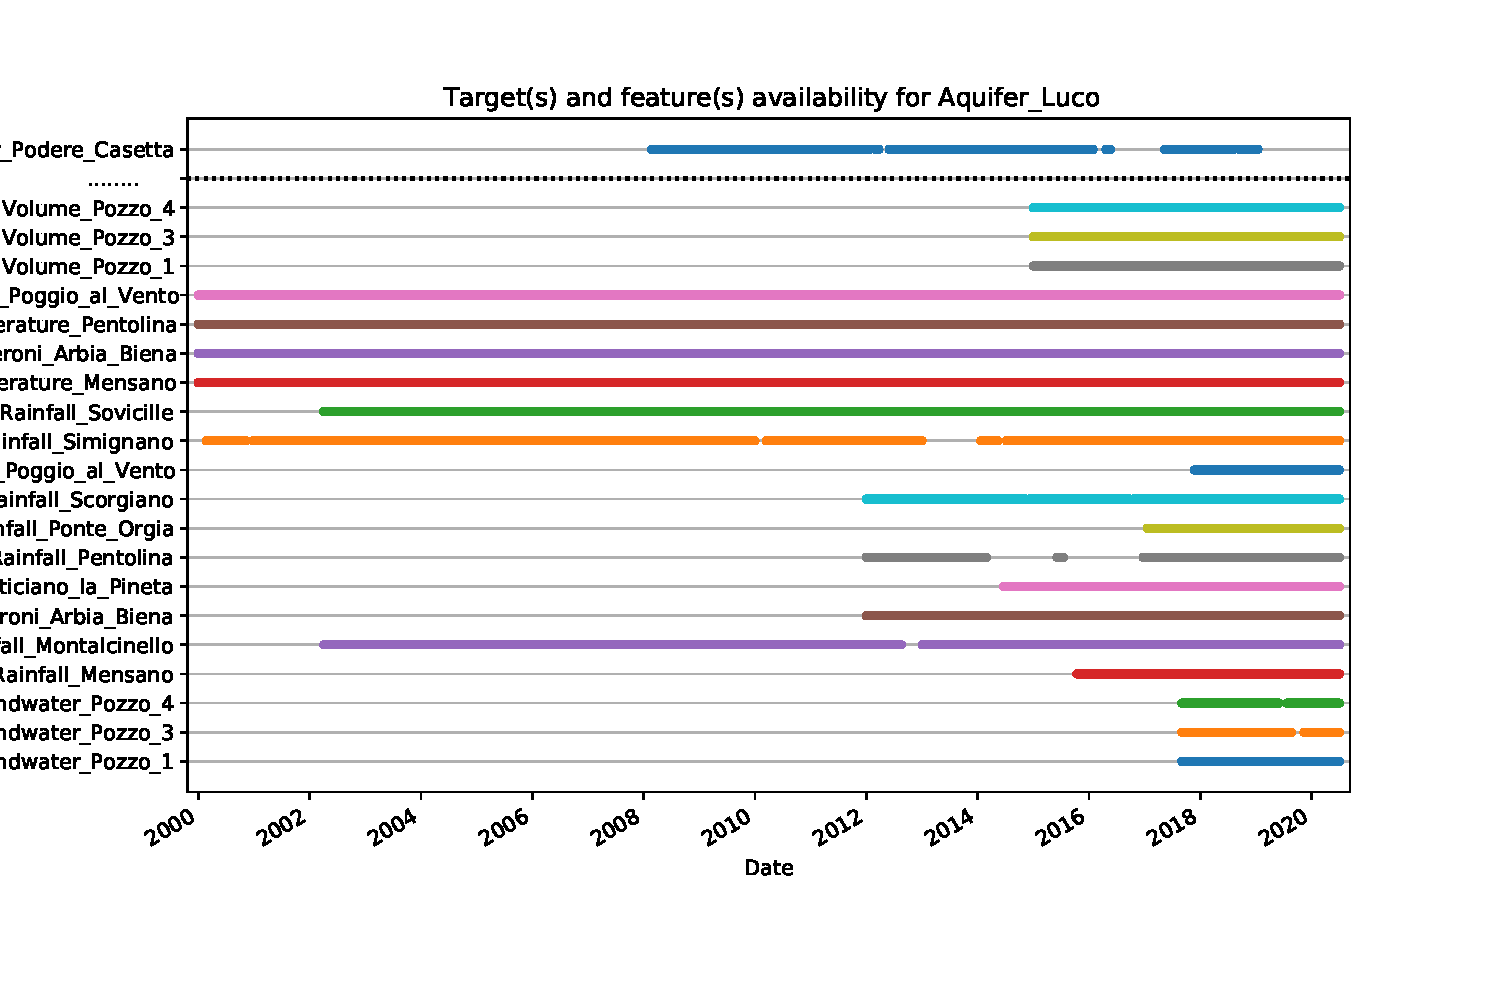
\includegraphics[width=0.9\textwidth]{figs/Aquifer_Luco.pdf}
\caption{Data availability for Aquifer Luco. The coloured horizontal bars indicate periods of data availability. The first measurement concerns the target value and the measurements below the dashed line concern features. Data collection of many features has started years after data collection of the target. Data collection of the target has been discontinued since over a year. There are hardly any time points in which both target and all features are collected.}
\label{fig:prep_missing_data}
\end{center}
\end{figure}

\begin{table}
\begin{center}
\resizebox{\textwidth}{!}{%
\begin{tabular}{ l || c ||  c c c c c c c}
Water body              	& Type 	& Depth to Groundwater 	& Flow Rate 	& Hydrometry	& Lake Level		& Volume 		& Rainfall 		& Temperature	\\
\hline
\hline
Auser                      		& A 		& 3T, 2F                       	&                	& 2F             	&				& 5F 		& 10			& 4F	 		\\
Petrignano               		& A 		& 2T                            	&                	& 1F             	&				& 1F  		& 1F 		& 2F			\\
Doganella                		& A 		& 9T                            	&                	&                 	&				& 8F 		& 2F 		& 2F	 		\\ 
Luco                       		& A 		& 1T, 3F                       	&                	&                 	&				& 3F 		& 10F 		& 4F	 		\\ 
Amiata                    		& WS  	& 3F                             	& 4T          	&			&				& 			& 4F 		& 3F 		\\
Madonna di Canneto 	& WS  	&                               	& 1T            	&                 	&				& 			& 1F 		& 1F			\\
Lupa                       		& WS  	&                               	& 1T            	&                   	&				& 			& 1F 		&  	  		\\
Arno                       		& R  		&                               	&             		& 1T              	&				& 			& 14F 		& 1F  		\\
Bilancino                 		& L 	 	&                               	& 1T            	&                   	& 1T				& 			& 5F 		& 1F 		\\
\end{tabular}}
\end{center}
\caption{The type of target(s) and features differs greatly per water body. Environmental features such as rainfall and temperature are available for all water bodies, whereas measurements such as volume and lake level are specific to one type of waterbody. The number indicates the number of targets (T) and features (F) specified in the column header. The type of water body is indicated as A (aquifer), WS (water spring), R (river) or L (lake).}
\label{tab:targets_features}
\end{table}



\begin{table}
\resizebox{\textwidth}{!}{%
\begin{tabular}{lrrrrrrr}
\toprule
Date        & Rainfall		  & Depth to Groundwater & Depth to Groundwater & Temperature & Temperature & Volume & Hydrometry \\
              &  Bastia Umbra &  P24 &  P25 &  Bastia Umbra &  Petrignano &  C10 Petrignano &  Fiume Chiascio Petrignano \\
\midrule
2009-01-01 &                    0.0 &                    -31.96 &                    -31.14 &                       5.2 &                     4.9 &             -24530.688 &                                   2.4 \\
2009-01-02 &                    0.0 &                    -32.03 &                    -31.11 &                       2.3 &                     2.5 &             -28785.888 &                                   2.5 \\
2009-01-03 &                    0.0 &                    -31.97 &                    -31.07 &                       4.4 &                     3.9 &             -25766.208 &                                   2.4 \\
2009-01-04 &                    0.0 &                    -31.91 &                    -31.05 &                       0.8 &                     0.8 &             -27919.296 &                                   2.4 \\
2009-01-05 &                    0.0 &                    -31.94 &                    -31.01 &                      -1.9 &                    -2.1 &             -29854.656 &                                   2.3 \\
2009-01-06 &                    0.0 &                    -31.89 &                    -31.00 &                      -0.7 &                    -0.7 &             -29124.576 &                                   2.3 \\
2009-01-07 &                    0.0 &                    -31.91 &                    -30.96 &                       1.5 &                    -0.3 &             -31173.120 &                                   2.3 \\
2009-01-08 &                    0.0 &                    -31.83 &                    -30.94 &                       4.3 &                     6.6 &             -30232.224 &                                   2.4 \\
2009-01-09 &                    0.9 &                    -31.80 &                    -30.93 &                       4.9 &                     4.8 &             -30597.696 &                                   2.3 \\
2009-01-10 &                    0.0 &                    -31.76 &                    -30.87 &                       1.9 &                     4.2 &             -31337.280 &                                   2.3 \\
\bottomrule
\end{tabular}}
\caption{Sample data extract for Aquifer Petrignano}
\label{tab:sample}
\end{table}


\subsection*{Exploratory Visualization}

Figure~\ref{fig:petrignano} shows the available data for aquifer Petrignano. A few observations can be made:

\begin{itemize}
\item The period in which the different measurements are available differs. While the target is avaialble from 2006 onwards, data collection for most of the features starts only in 2009. For most of the water bodies a similar misalignment between data availability of target and features is observed, which is also indicated by the small percentage of \emph{complete} records as already mentioned in the previous section.
\item A yearly pattern is seen in the target variable. This can be understood as water bodies fill in autumn and winter when more water enters the bodies then is being utilised, while in spring and autumn water levels drop. 
\item Invalid readings occur in the measurements of hytrometry and temperature. Invalid reading can be recognized by many subsequent readings with the value $0$. Additionally, occasionally a data point is missing. These datapoints can be easitly interpolated. In case data is missing for a longer period of time, as is the case with the invalid reading, data cannot be interpolated.
\item There is often a strong correlation between different measurements of the same type. For example, the temperature and the depth to groundwater each have two measurements for aquifer Petrignano. As can be seen from Fig~\ref{fig:petrignano} these follow the same pattern. It must be noted that although different temperature measurments always follow the same pattern, this does not always hold true for the other types of measurements. For example, aquifer Auser has three measurements of depth to groundwater which each exhibit a very distinct pattern.  
\end{itemize}

\begin{figure}[p]
     \centering
     \begin{subfigure}
         \centering
         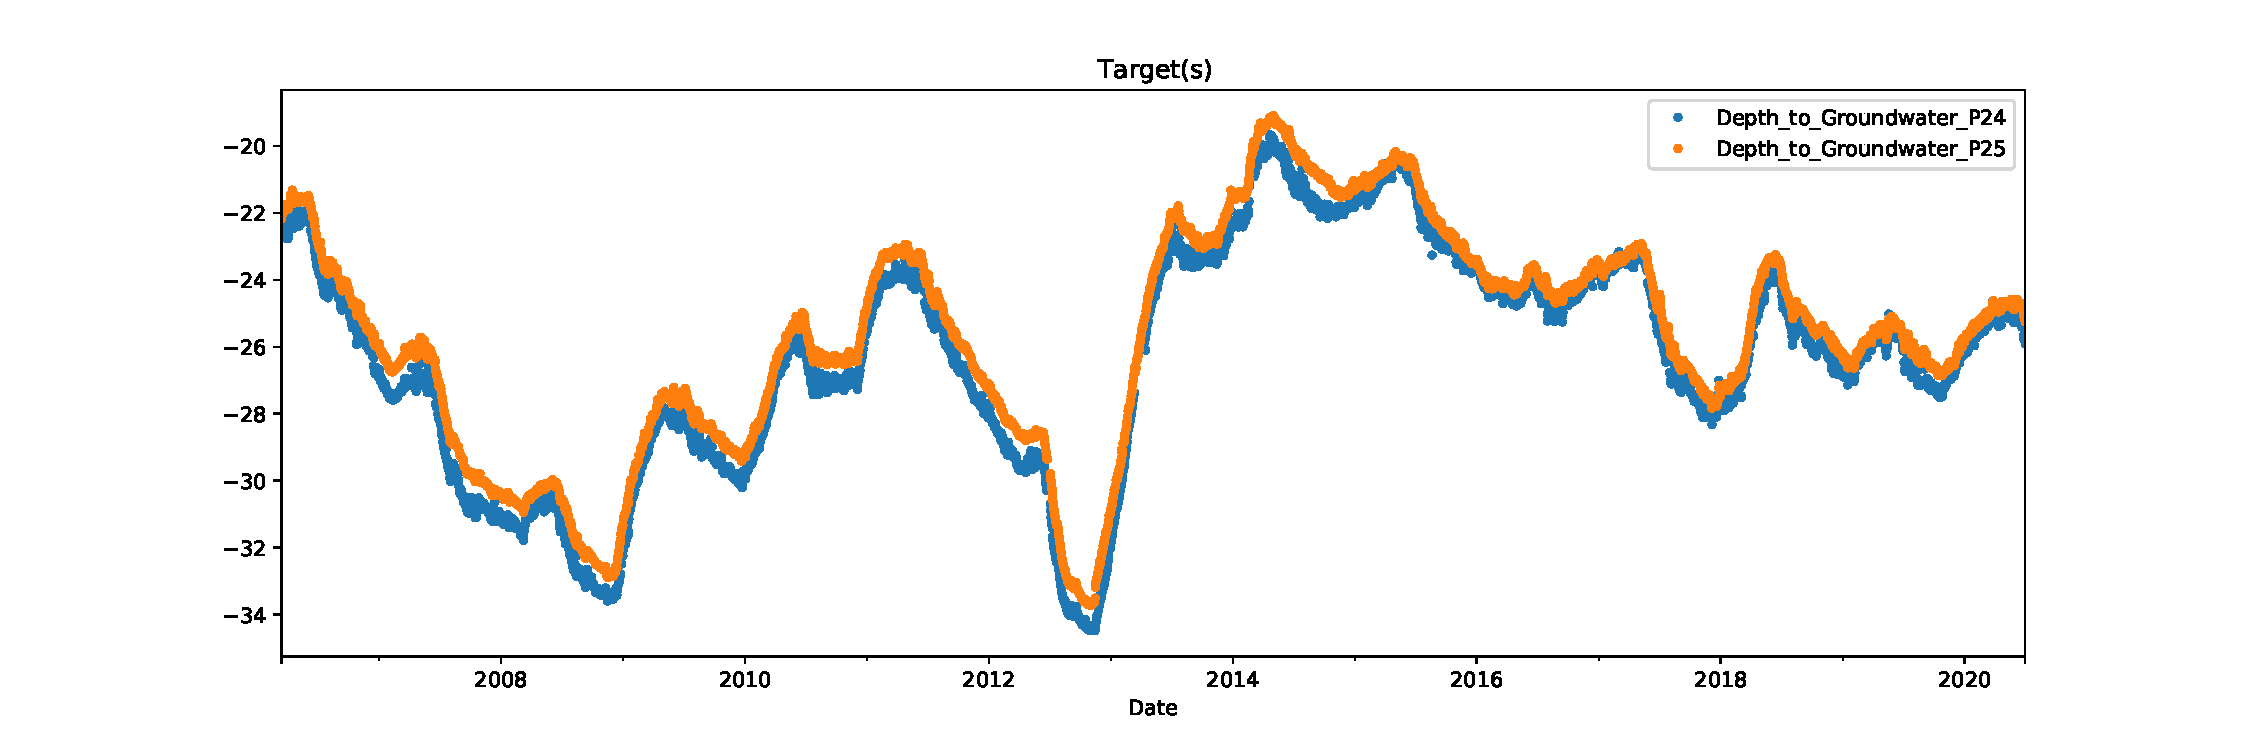
\includegraphics[width=0.8\textwidth]{figs/Aquifer_Petrignano_target.pdf}
     \end{subfigure}
% 
     \begin{subfigure}
         \centering
         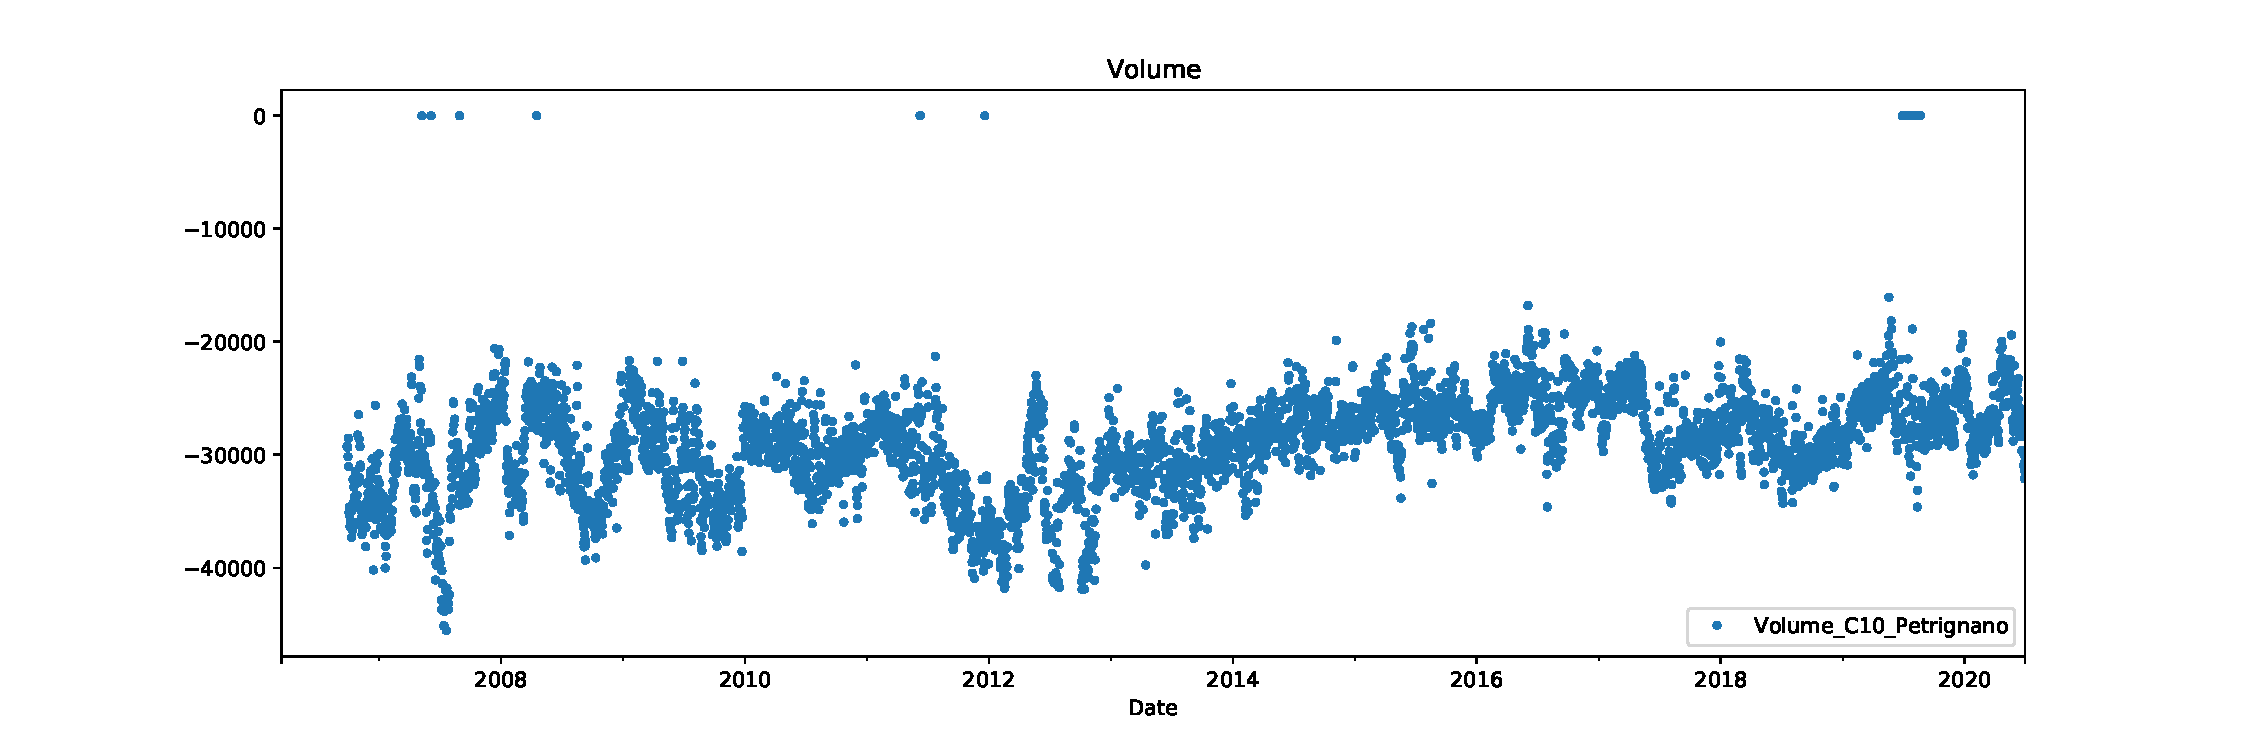
\includegraphics[width=0.8\textwidth]{figs/Aquifer_Petrignano_Volume.pdf}
     \end{subfigure}
% 
     \begin{subfigure}
         \centering
         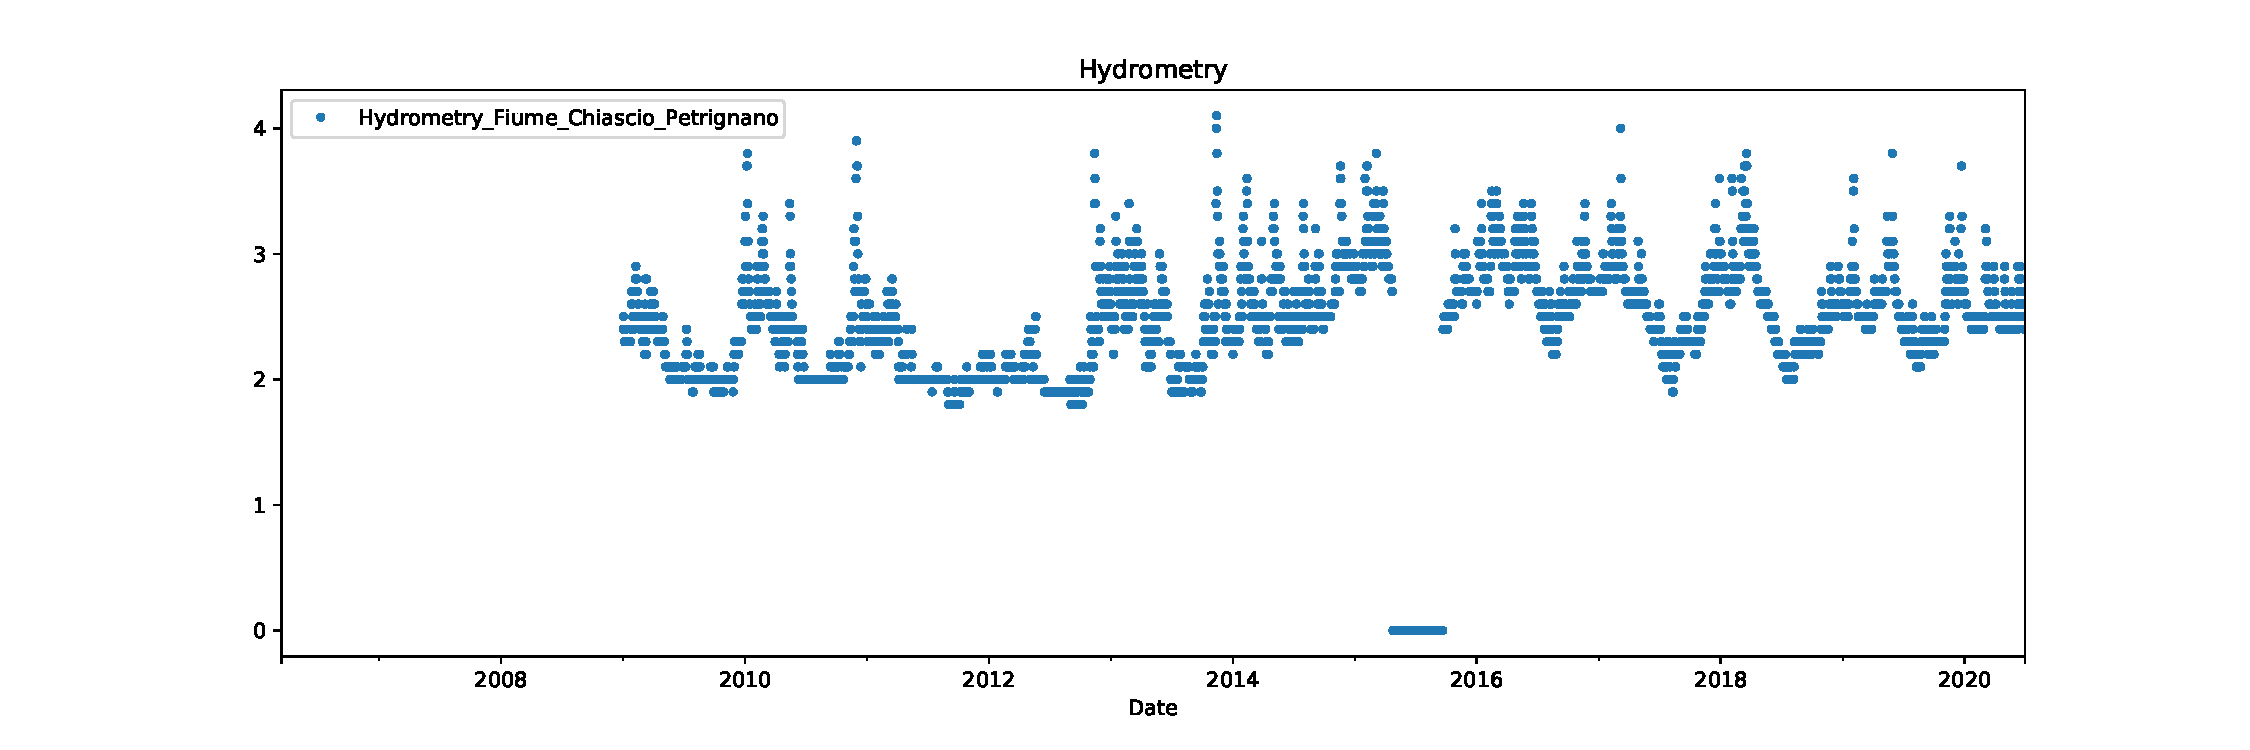
\includegraphics[width=0.8\textwidth]{figs/Aquifer_Petrignano_Hydrometry.pdf}
     \end{subfigure}
%
     \begin{subfigure}
         \centering
         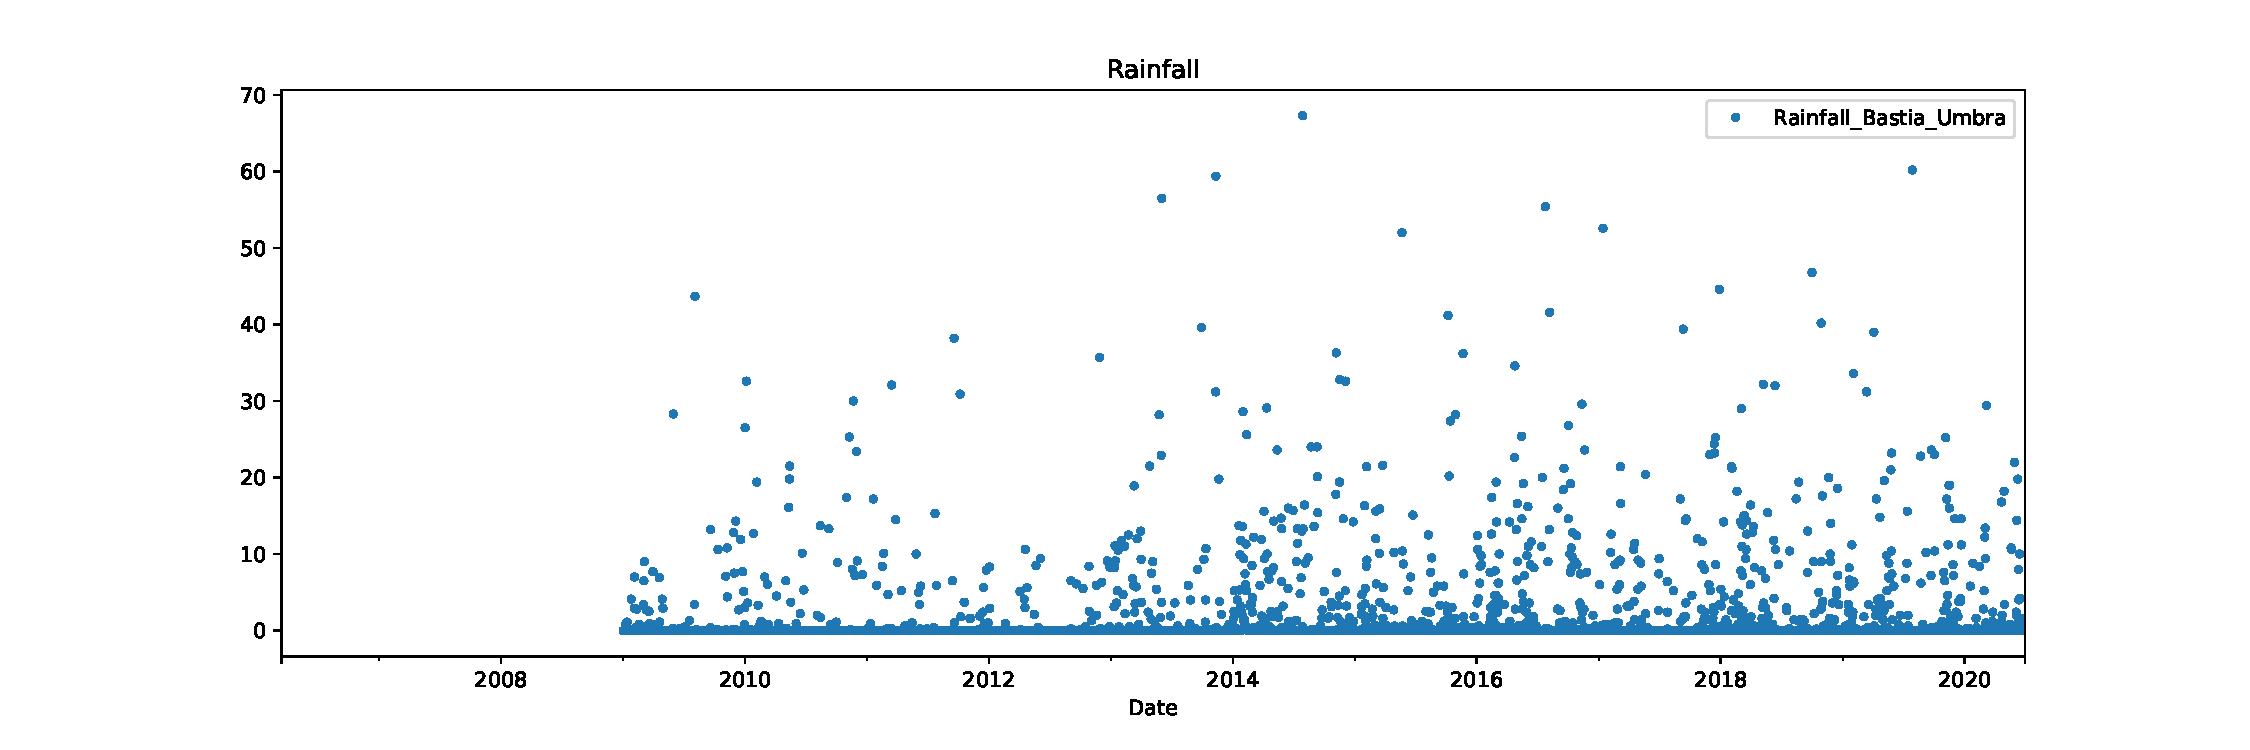
\includegraphics[width=0.8\textwidth]{figs/Aquifer_Petrignano_Rainfall.pdf}
     \end{subfigure}
%
     \begin{subfigure}
         \centering
         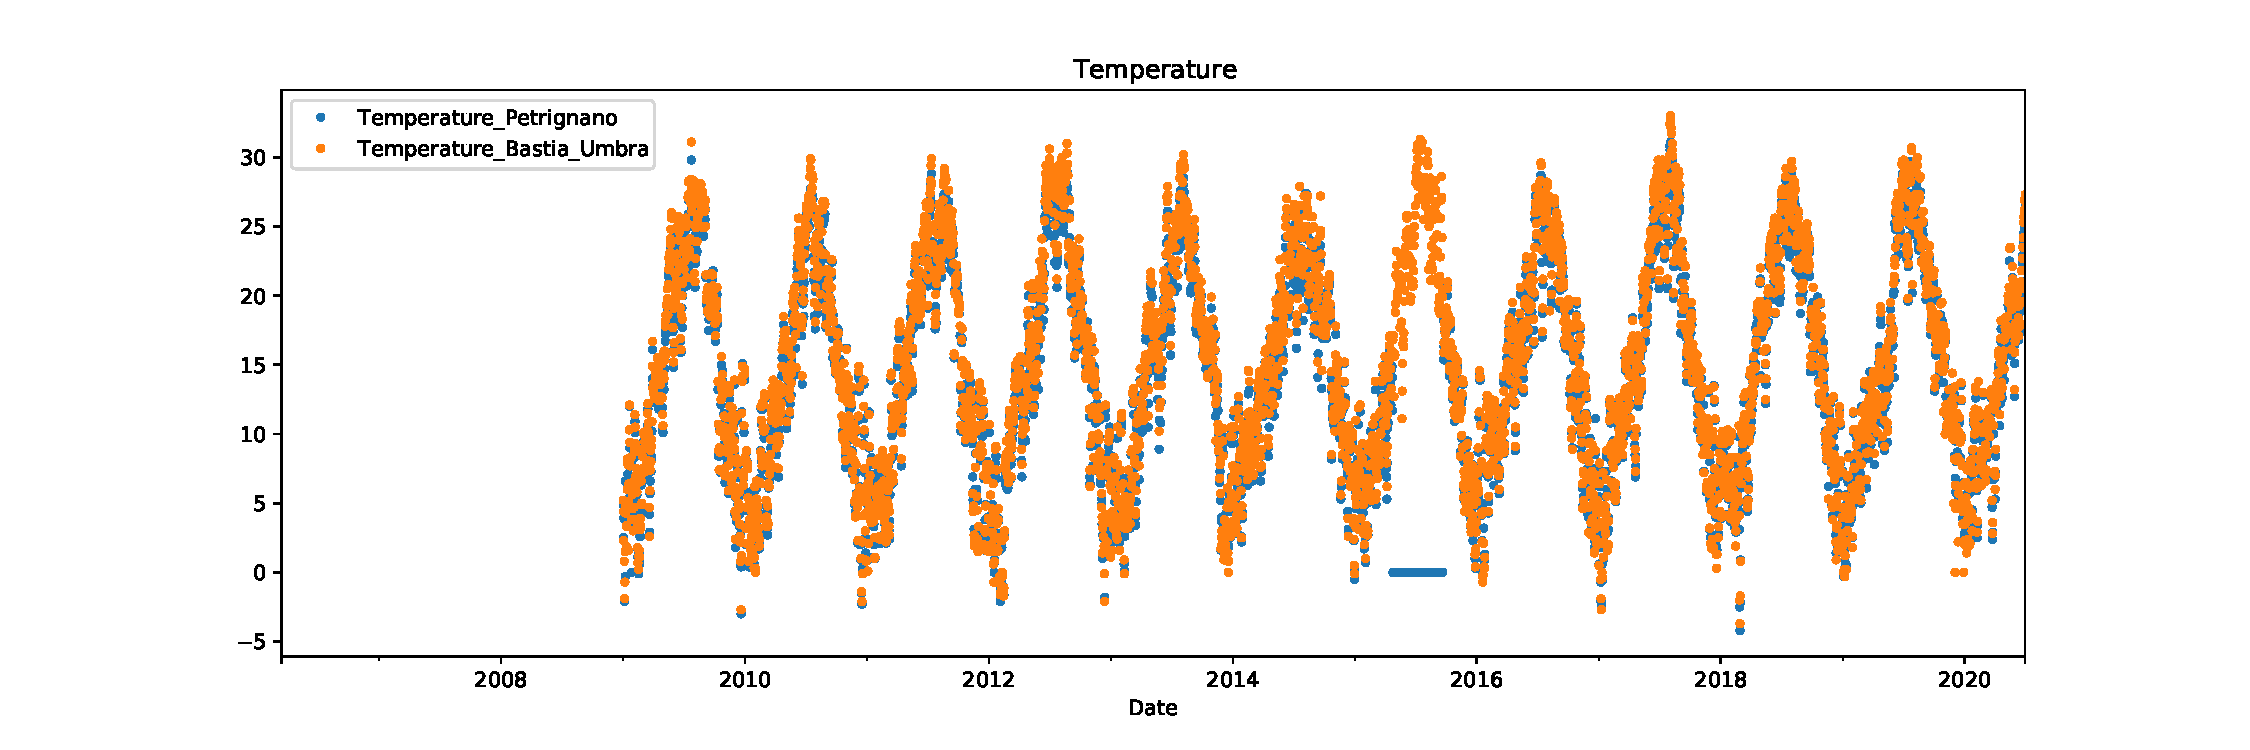
\includegraphics[width=0.8\textwidth]{figs/Aquifer_Petrignano_Temperature.pdf}
     \end{subfigure}
     \caption{Measurements available for aquifer Petrignano. From top to bottom: the target variables Depth to Groundwater and the features Volume, Hydrometry Rainfall, Temperature.}
     \label{fig:petrignano}
\end{figure}


% Add two more examples:
% flow rate lake (target) seems to be controlled by a water lock. It is a bit hard to predict here when human intervention will happen and to what level the water lock is set in that case.
% offset in hydrometry readings after 2011

\subsection*{Algorithms and Techniques}

In any machine learning problem is it vital to select the correct features. Three statistical methods are used to select features:
\begin{itemize} 
\item Pearson correlation~\cite{pearson}, the most commonly used correlation coefficient. However, this coefficient captures only linear relations.
\item $\phi_k$ correlation~\cite{phik}, a recently introduced correlation coefficient which works alike for interval, ordinal and categorical variables. Moreover, this correlation coefficient does caption non-linear relations.
\item Predictive Power Score (PPS)~\cite{pps}, a method based on training a RandomForest based on one feature. The trained model is compared to a \emph{naive} model in order to construct the PPS. As a RandomForest is used this method captures non-linear relationships. 
\end{itemize}

The selection of features is often an iterative process. Although the above mentioned methods provide a means of doing a first selection, a manual refinement is necessary. In this refinement correlations between the different features can be taken into account as many of the provided features are strongly correlated.

As historic water level and water flow measurements are recorded it is possible to approach this task using supervised learning. In order to capture complex relations between features and target, a regression model which can capture non-linear relations might be preferred, such as Sklearn's RandomForestRegressor or MLPRegressor. Sklearn's common model interface allows us to easily explore several models. Furthermore, XGBoost, which has proven to be a winning algorithm in many previous Kaggle competitions, could offer a solution which is worth exploring. 

Cross validation is used for model selection and hyperparameter tuning. As the data concerns a time series and only predictions for the future are relevant, an out of sample cross validation strategy is designed as illustrated in Fig.~\ref{fig:kfolds_cv} left. The length of the training period is experimentally determined. The size of the prediction horizon is not defined in the problem statement~\cite{kaggle} and will be taken as 1 week. The testing period is taken as 30 days. Note that the number of folds depends on the size of the dataset and varies between the different water bodies.

\begin{figure}[htb]
     \centering
     \begin{subfigure}
         \centering
         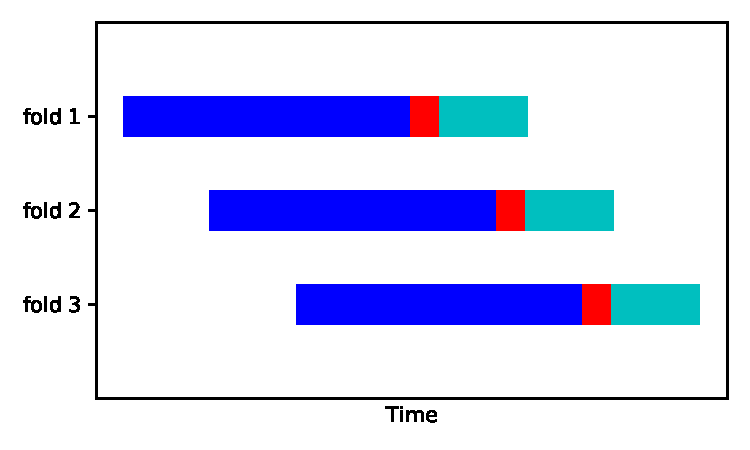
\includegraphics[width=0.45\textwidth]{figs/kfolds.pdf}
     \end{subfigure}
% 
     \begin{subfigure}
         \centering
         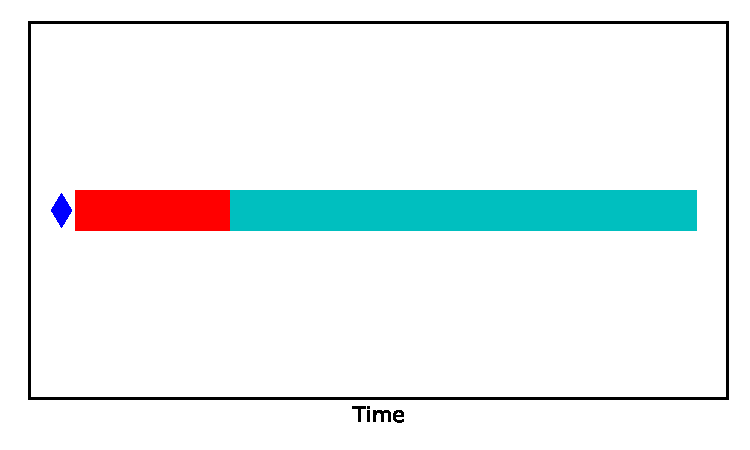
\includegraphics[width=0.45\textwidth]{figs/benchmark.pdf}
     \end{subfigure}
\caption{Left -- Kfolds cross validation schema taking into account a prediction horizon (red). The blue (cyan) bar indicates the training (testing) period. Note that the training and testing period are separated by the prediction horizon. Right -- As benchmark model the last known value of the target before the prediction horizon is used, as indicated with the blue diamond.}
\label{fig:kfolds_cv}
\end{figure}

Depending on the final model of choice a feature importance method need to be selected. For a simple linear model the coeficients give direct insight in the importance of the different features. For the RandomForestRegressor a feature importance method is implemented in Sklearn and readily available for use. Care needs to be taken as the standard feature importance method is biased towards high cardinality features. The permutation importance is not sensitive to cardinality and can be used as an alternative. Moreover, this method can be applied for any Sklearn model.

\subsection*{Benchmark}

The base model is chosen as the last known value of the target before the prediction horizon, as illustrated in Fig.~\ref{fig:kfolds_cv} right. Especially for a relative short prediction horizon, such as a week, it might be challenging to improve upon this simple model by including other features due to the slowly changing nature of the target. Model performance metrics of the base model for a prediction horizon of 7, 30 and 60 days are listed in Tabs.~\ref{tab:bm7}-\ref{tab:bm60}. For a longer prediction horizon it the accuracy of the model performance of the base model decreases. 

\begin{table}[p]
\resizebox{\textwidth}{!}{%
\begin{tabular}{lllll}
\toprule
{} &                  r2 &                 rmse &                mae &               mape \\
\midrule
Aquifer\_Auser\_Depth\_to\_Groundwater\_SAL      &  $ -0.95 \pm 0.88 $ &    $ 0.03 \pm 0.06 $ &  $ 0.12 \pm 0.09 $ &  $ 0.02 \pm 0.02 $ \\
Aquifer\_Auser\_Depth\_to\_Groundwater\_COS      &  $ -0.41 \pm 0.96 $ &    $ 0.06 \pm 0.10 $ &  $ 0.19 \pm 0.12 $ &  $ 0.03 \pm 0.02 $ \\
Aquifer\_Auser\_Depth\_to\_Groundwater\_LT2      &  $ -0.59 \pm 0.76 $ &    $ 0.01 \pm 0.00 $ &  $ 0.05 \pm 0.02 $ &  $ 0.00 \pm 0.00 $ \\
Aquifer\_Petrignano\_Depth\_to\_Groundwater\_P24 &  $ -0.49 \pm 0.71 $ &    $ 0.07 \pm 0.06 $ &  $ 0.21 \pm 0.09 $ &  $ 0.01 \pm 0.00 $ \\
Aquifer\_Petrignano\_Depth\_to\_Groundwater\_P25 &  $ -0.37 \pm 0.80 $ &    $ 0.03 \pm 0.04 $ &  $ 0.14 \pm 0.07 $ &  $ 0.01 \pm 0.00 $ \\
Lake\_Bilancino\_Lake\_Level                   &  $ -0.83 \pm 2.79 $ &    $ 0.21 \pm 0.54 $ &  $ 0.27 \pm 0.21 $ &  $ 0.00 \pm 0.00 $ \\
Lake\_Bilancino\_Flow\_Rate                    &    $ -inf \pm inf $ &  $ 16.76 \pm 53.88 $ &  $ 1.28 \pm 2.15 $ &  $ 0.39 \pm 0.48 $ \\
River\_Arno\_Hydrometry\_Nave\_di\_Rosano        &  $ -1.55 \pm 2.51 $ &    $ 0.30 \pm 0.48 $ &  $ 0.29 \pm 0.27 $ &  $ 0.16 \pm 0.11 $ \\
\bottomrule
\end{tabular}
}
\caption{Model evaluation metrics for the base model with a prediction horizon of 7 days.}
\label{tab:bm7}
\end{table}

\begin{table}[p]
\resizebox{\textwidth}{!}{%
\begin{tabular}{lllll}
\toprule
{} &                      r2 &                 rmse &                mae &               mape \\
\midrule
Aquifer\_Auser\_Depth\_to\_Groundwater\_SAL      &      $ -8.14 \pm 9.50 $ &    $ 0.18 \pm 0.32 $ &  $ 0.27 \pm 0.23 $ &  $ 0.05 \pm 0.05 $ \\
Aquifer\_Auser\_Depth\_to\_Groundwater\_COS      &    $ -17.28 \pm 36.43 $ &    $ 0.70 \pm 1.02 $ &  $ 0.64 \pm 0.42 $ &  $ 0.11 \pm 0.08 $ \\
Aquifer\_Auser\_Depth\_to\_Groundwater\_LT2      &      $ -5.35 \pm 5.87 $ &    $ 0.02 \pm 0.02 $ &  $ 0.13 \pm 0.06 $ &  $ 0.01 \pm 0.00 $ \\
Aquifer\_Petrignano\_Depth\_to\_Groundwater\_P24 &      $ -6.29 \pm 5.78 $ &    $ 0.37 \pm 0.44 $ &  $ 0.48 \pm 0.29 $ &  $ 0.02 \pm 0.01 $ \\
Aquifer\_Petrignano\_Depth\_to\_Groundwater\_P25 &     $ -9.99 \pm 15.11 $ &    $ 0.31 \pm 0.53 $ &  $ 0.42 \pm 0.33 $ &  $ 0.02 \pm 0.01 $ \\
Lake\_Bilancino\_Lake\_Level                   &  $ -101.37 \pm 475.53 $ &    $ 1.64 \pm 3.21 $ &  $ 0.91 \pm 0.79 $ &  $ 0.00 \pm 0.00 $ \\
Lake\_Bilancino\_Flow\_Rate                    &        $ -inf \pm inf $ &  $ 25.65 \pm 59.41 $ &  $ 2.18 \pm 2.77 $ &  $ 1.22 \pm 2.08 $ \\
River\_Arno\_Hydrometry\_Nave\_di\_Rosano        &     $ -8.53 \pm 17.22 $ &    $ 0.45 \pm 0.65 $ &  $ 0.39 \pm 0.33 $ &  $ 0.23 \pm 0.16 $ \\
\bottomrule
\end{tabular}
}
\caption{Model evaluation metrics for the base model with a prediction horizon of 30 days.}
\label{tab:bm30}
\end{table}

\begin{table}[p]
\resizebox{\textwidth}{!}{%
\begin{tabular}{lllll}
\toprule
{} &                        r2 &                 rmse &                mae &               mape \\
\midrule
Aquifer\_Auser\_Depth\_to\_Groundwater\_COS      &      $ -30.02 \pm 43.97 $ &    $ 1.78 \pm 2.61 $ &  $ 1.01 \pm 0.80 $ &  $ 0.18 \pm 0.17 $ \\
Aquifer\_Auser\_Depth\_to\_Groundwater\_LT2      &      $ -18.34 \pm 19.13 $ &    $ 0.07 \pm 0.08 $ &  $ 0.23 \pm 0.12 $ &  $ 0.02 \pm 0.01 $ \\
Aquifer\_Auser\_Depth\_to\_Groundwater\_SAL      &      $ -24.63 \pm 45.97 $ &    $ 0.34 \pm 0.62 $ &  $ 0.38 \pm 0.40 $ &  $ 0.08 \pm 0.09 $ \\
Aquifer\_Petrignano\_Depth\_to\_Groundwater\_P24 &      $ -22.69 \pm 33.40 $ &    $ 1.05 \pm 1.46 $ &  $ 0.82 \pm 0.55 $ &  $ 0.03 \pm 0.02 $ \\
Aquifer\_Petrignano\_Depth\_to\_Groundwater\_P25 &     $ -62.19 \pm 170.06 $ &    $ 1.00 \pm 1.70 $ &  $ 0.77 \pm 0.61 $ &  $ 0.03 \pm 0.03 $ \\
Lake\_Bilancino\_Flow\_Rate                    &          $ -inf \pm inf $ &  $ 28.94 \pm 64.93 $ &  $ 2.84 \pm 3.59 $ &  $ 1.68 \pm 2.47 $ \\
Lake\_Bilancino\_Lake\_Level                   &  $ -1562.05 \pm 6558.16 $ &    $ 3.63 \pm 3.53 $ &  $ 1.56 \pm 0.90 $ &  $ 0.01 \pm 0.00 $ \\
River\_Arno\_Hydrometry\_Nave\_di\_Rosano        &      $ -31.35 \pm 66.90 $ &    $ 0.76 \pm 1.09 $ &  $ 0.54 \pm 0.43 $ &  $ 0.32 \pm 0.23 $ \\
\bottomrule
\end{tabular}
}
\caption{Model evaluation metrics for the base model with a prediction horizon of 60 days.}
\label{tab:bm60}
\end{table}

\FloatBarrier


\section{Methodology}

\subsection*{Preprocessing}

% cleaning

\subsubsection*{Data cleaning}

In order to create a dataset suitable for modelling the following preprocessing steps are taken to clean the data:

%offset hytrometry reading!

\begin{itemize}
\item Select water bodies for which there is a reasonable amount of \emph{complete} records
\item Select the time period in which records are complete
\item Set dtype to datetime for the Date column and to float for all other columns
\item Replace invalid readings with NaN
\item Interpolate missing data where only one subsequent data point in missing
\item Take the absolute value of the flow rate values
\end{itemize}

% feature engineering
\subsubsection*{Feature engineering}

Typically water bodies fill in autumn and winter when more water enters the bodies then is being utilised, while in spring and autumn water levels drop, giving rise to a seasonal pattern in the water availability. In order to provide the model with seasonal information the features \emph{month} is created based on the Date column. As the proposed model only consumes numerical data the month is dummy encoded. 

From Fig.~\ref{fig:petrignano} (top) it is evident that there are trends in water availability which span over several years of time: for some subsequent years the water body slowly empties, while in other subsequent years the availability of water increases. In order to capture these trends \emph{lagged} features are introduced, which compare the target value just before the prediction horizon with a value measured in the past. To be less sensitive to fluctuations, the values are averaged over a period of time.

Intuitively one can argue that rain water does not necessarily become readily available in a water body. Depending on the distance from the area with rain to the water body there could be a period of time between the rainfall and the water entering the water body. For aquifers it might take time for the water to penetrate the ground and reach the aquifer. For rivers and lakes, water might need to be transported to the water body through canals or smaller rivers. In order to capture a potential delay, lagged features are created for rainfall. Both rainfall and temperature measurements are often provided for several geographical location. Different temperature (rainfall) measurements are typically highly correlated, therefore one temperature (rainfall) features is constructed based on all the provided measurements. Long periods with high temperatures could have an effect on water temperature and therefore on the amount of evaporation from a lake or river. Lagged features are created to capture this information.

Volume and hydrometry are related to the water body itself and any change in those features is expected to have a direct effect. Although the seasonal pattern can be observed in the hydrometry measurements, no clear trends are observed. The use of lagged features of these types seems therefore less promising.  Volume is a feature that indicates the water consumption from the water body, and as such is a result of a human action. Although the total water consumption is related to the temperature, it is up to Acea to determine which water body to utilise to provide the necessary water for daily consumption. Effects of this human influence can be seen in Fig.~\ref{fig:petrignano} (middle), where volume clearly follows a seasonal pattern from 2007 to 2013, then steadily decreases until 2017 presumably to increase the ground water level which experienced a dramatic drop in 2012-2013, followed by another period where a seasonal effect is visible. Although water volume for Aquifer Petrignano seems to follow a consumption pattern  which different volume intake for each subsequent days, there are also aquifers where volume is set on a monthly basis and remains fixed throughout the month. Any unexpected weather conditions resulting is larger or smaller water intake compared to the expectation for that month, must therefore be compensated by the other water bodies. This gives rise to the question whether it is possible to model  the water availablity of one individual water body, or whether the system of water bodies is interconnected and should be modelled as one big system.

After the creation of lagged features, all records in for which at least one feature or the target is NaN are dropped.


\subsubsection*{Feature selection}

The most straightforward feature selection is based on Pearson correlation. As the Pearson correlation only captures linear correlations, the feature selection is extended by the introduction of the $\phi_k$ correlation and PPS score. These methods allow to capture non-linear relations and might therefore select features which are not be identified as correlated by the Pearson correlation.

As lagged features are created in the feature engineering step it is not surprising to find highly correlated features, as shown in Fig.~\ref{fig:corr_auser}. Typically there is some overlap between the different feature selection methods but the PPS method selects significantly fewer features, even though the selection threshold is set rather low (below 0.5). The $\phi_k$ correlation selects more feature than the Pearson correlation (which comparable threshold) which might be explained by the presence of a non-linear relation. In other cases the $\phi_k$ correlation selects fewer features, which can be explained by the fact the $\phi_k$ correlation correlation treats every feature as categorical and therefore bins the feature. It might be that the number of bins (default value = 10) is insufficient to caption the variation the feature, leading to a smaller correlation. It is a priori unclear which feature selection method works best. This will be explored by creating models based on the different feature sets and comparing their performance. 

\begin{figure}
     \centering
     \begin{subfigure}
         \centering
         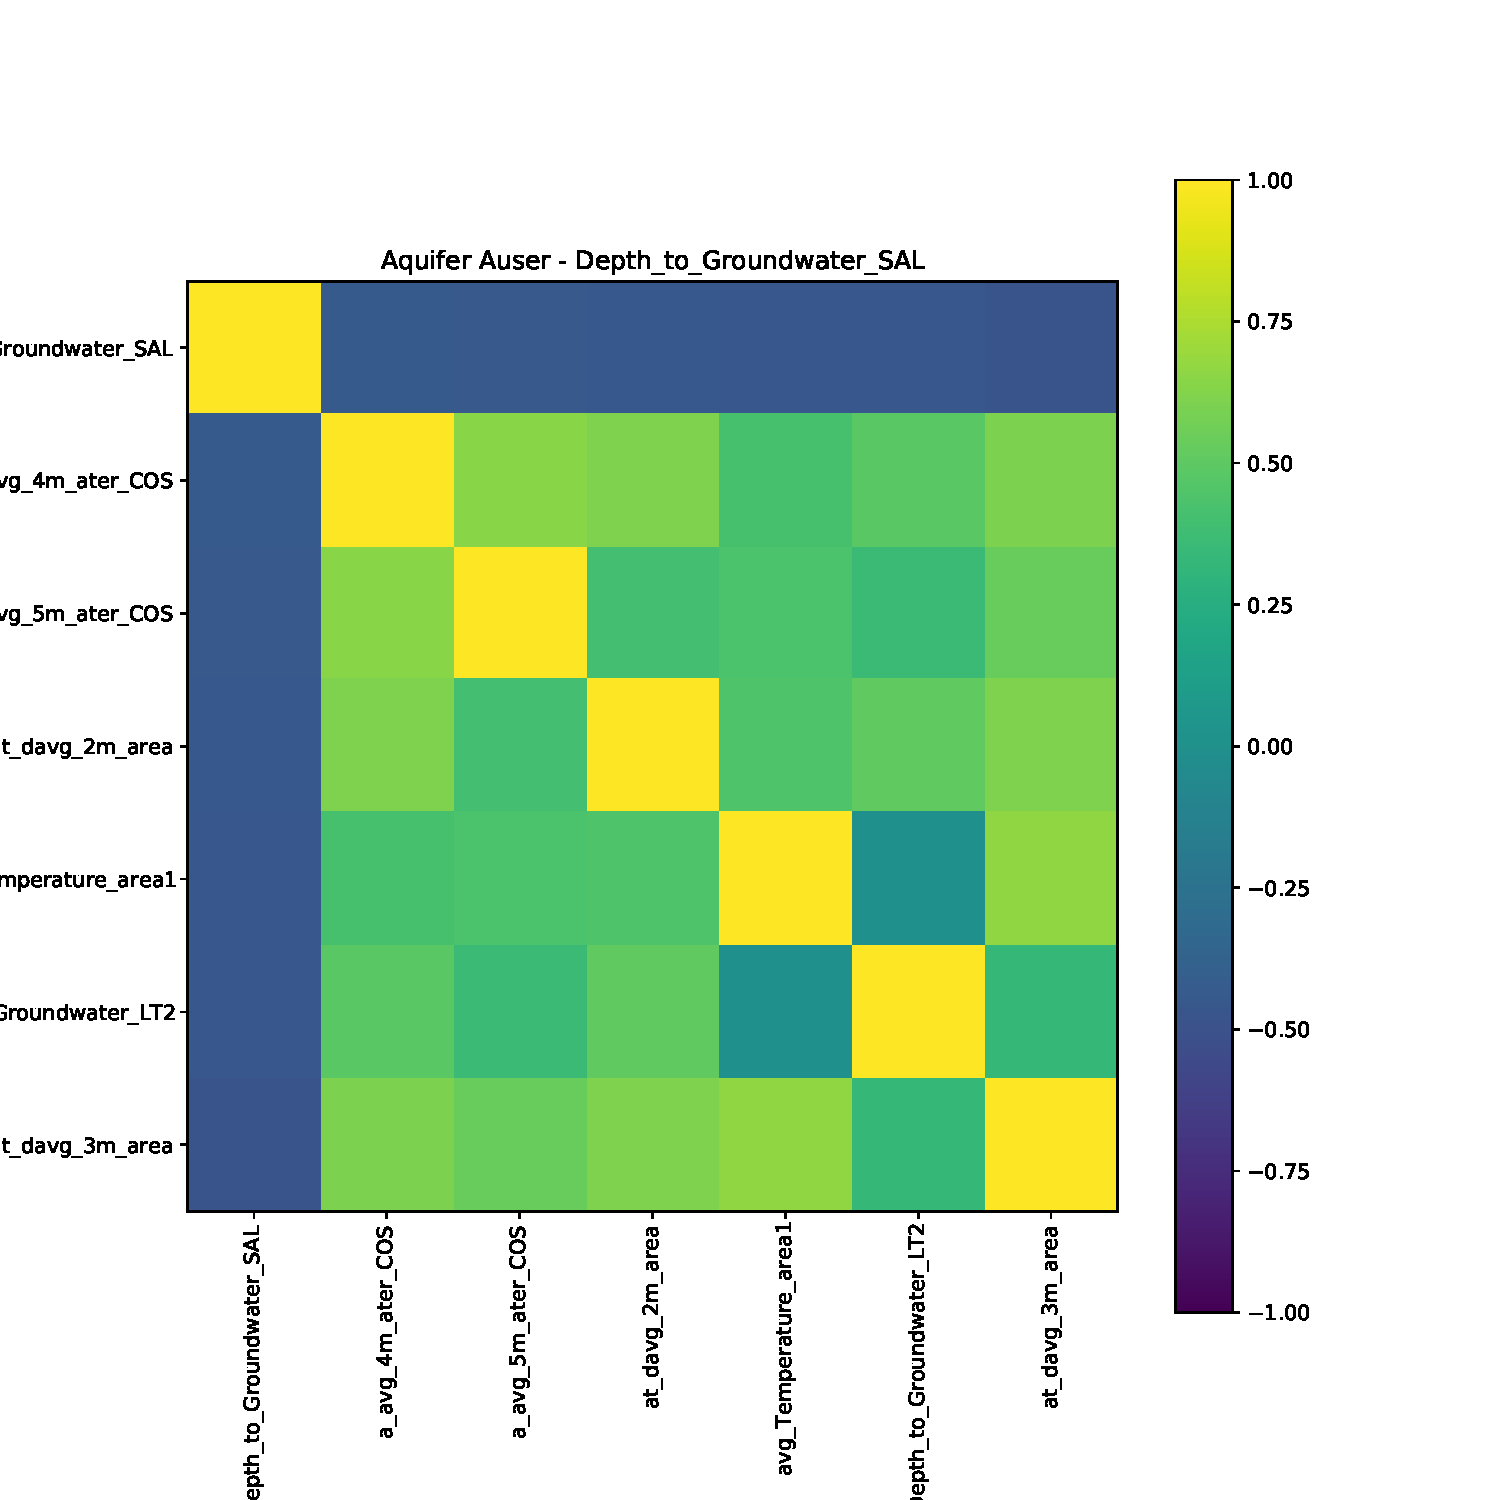
\includegraphics[width=0.45\textwidth]{figs/corr_Aquifer_Auser_Depth_to_Groundwater_SAL_pearson.pdf}
     \end{subfigure}
% 
     \begin{subfigure}
         \centering
         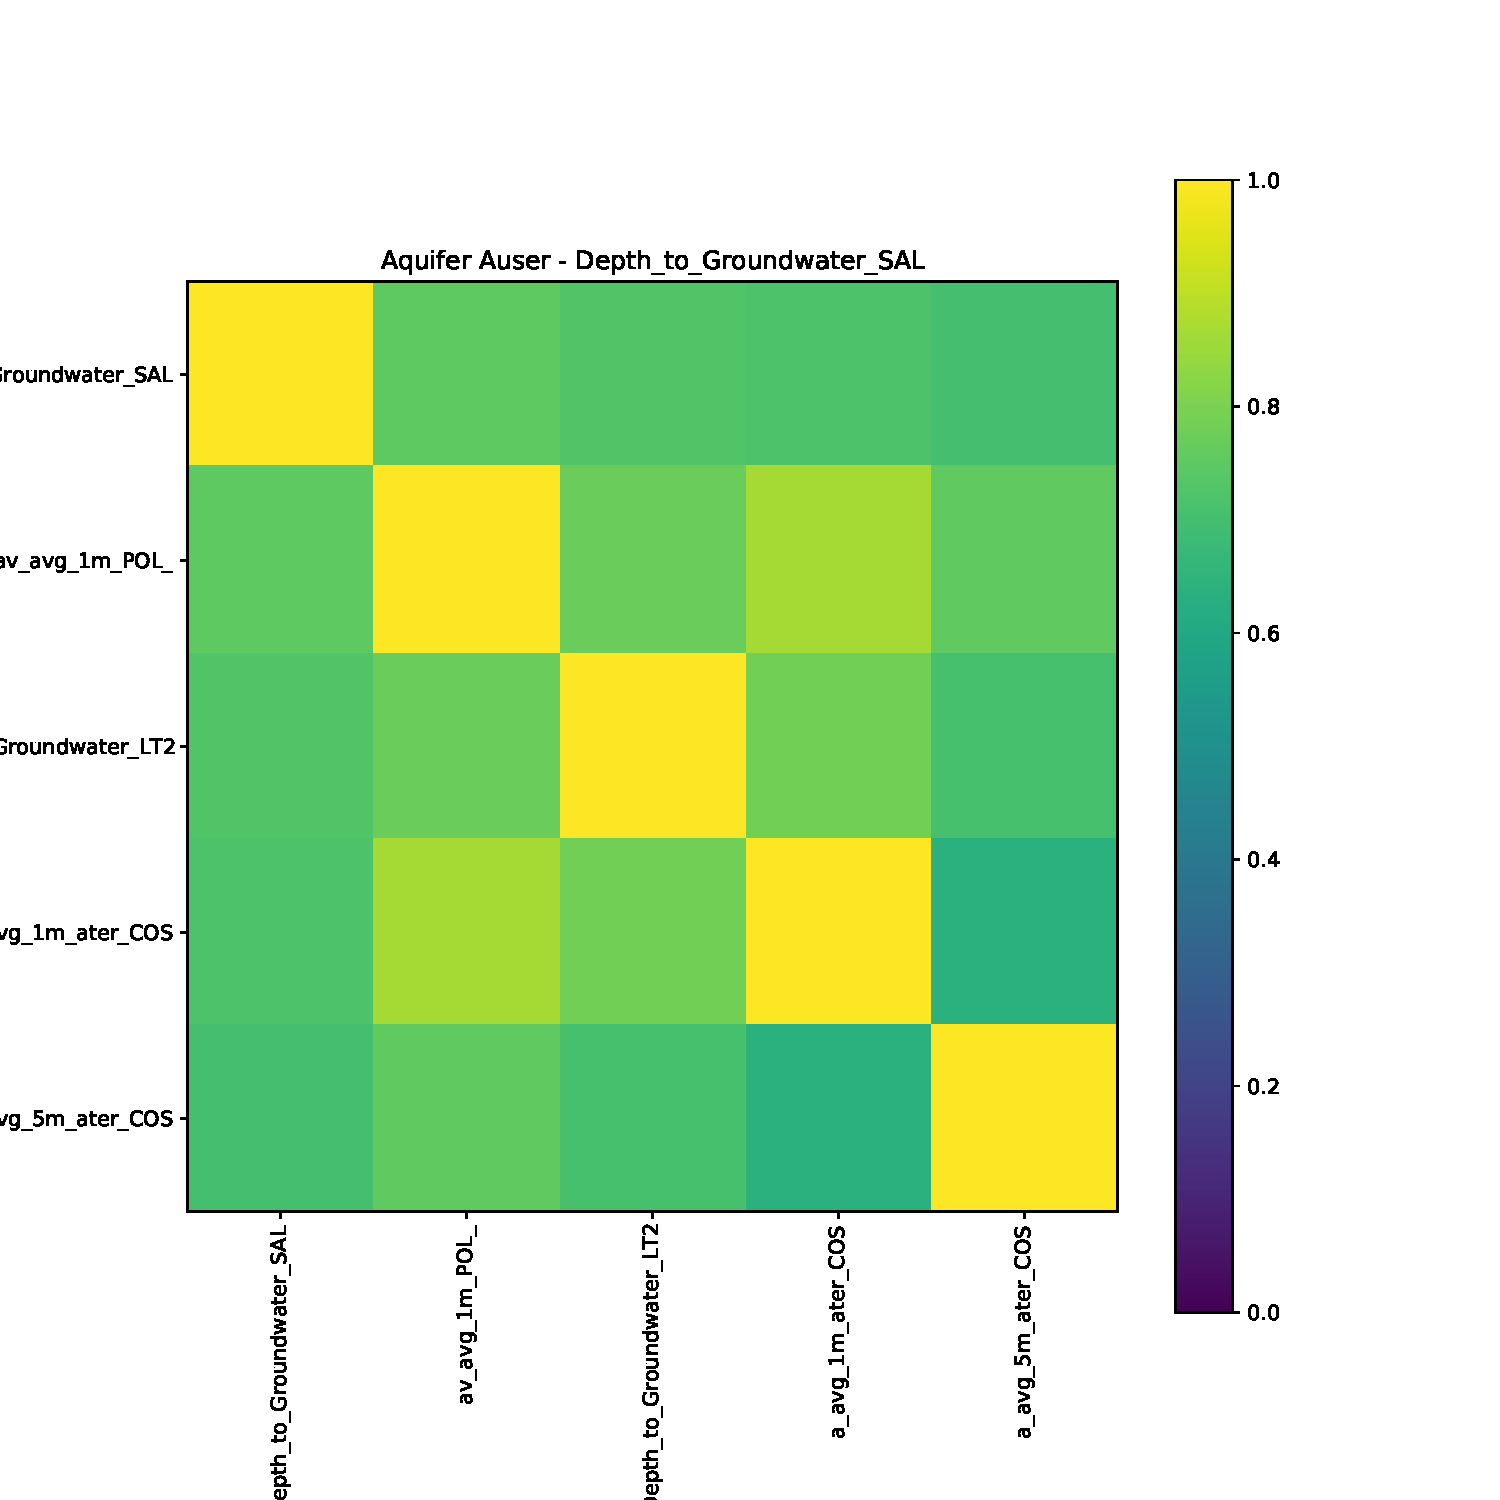
\includegraphics[width=0.45\textwidth]{figs/corr_Aquifer_Auser_Depth_to_Groundwater_SAL_phik.pdf}
     \end{subfigure}
%
     \begin{subfigure}
         \centering
         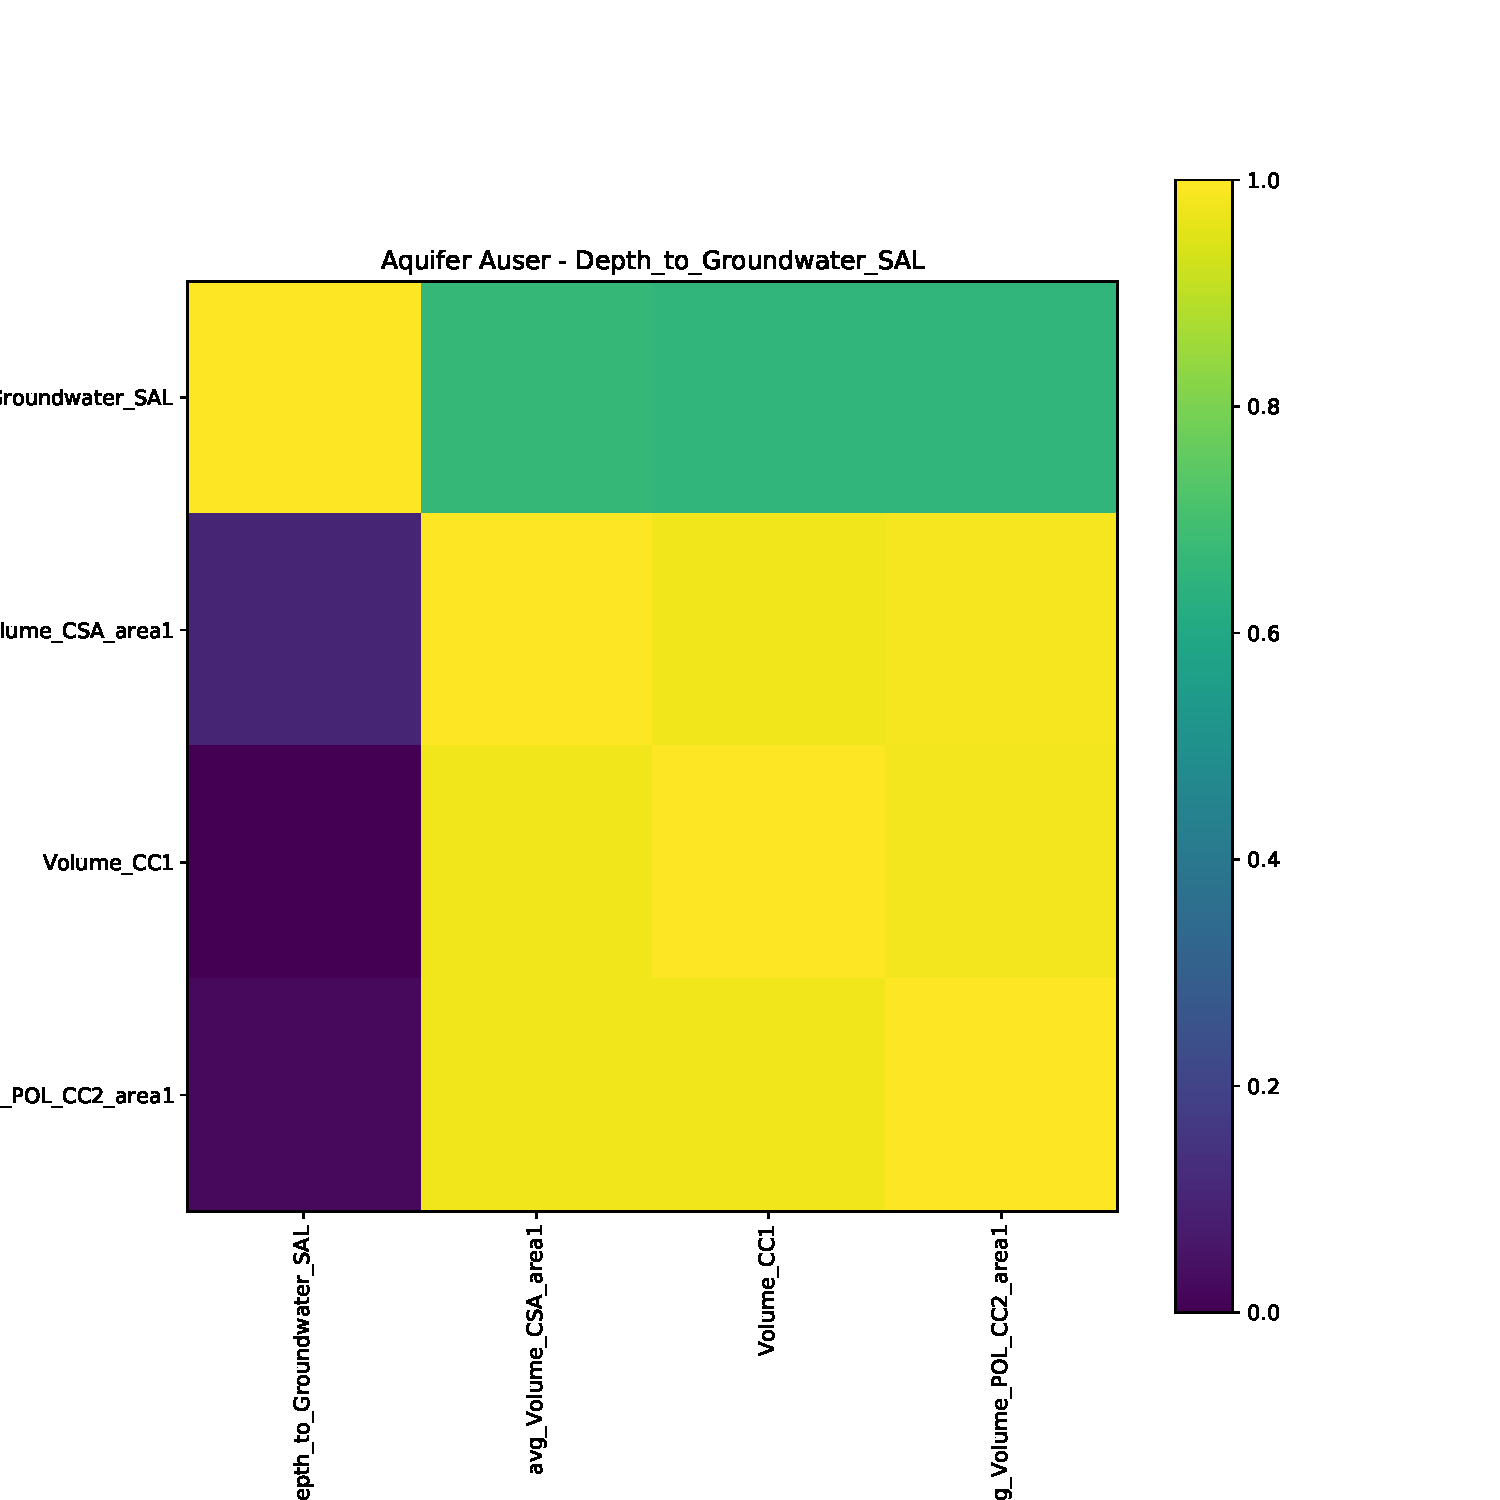
\includegraphics[width=0.45\textwidth]{figs/corr_Aquifer_Auser_Depth_to_Groundwater_SAL_pps.pdf}
     \end{subfigure}
% 
     \begin{subfigure}
         \centering
         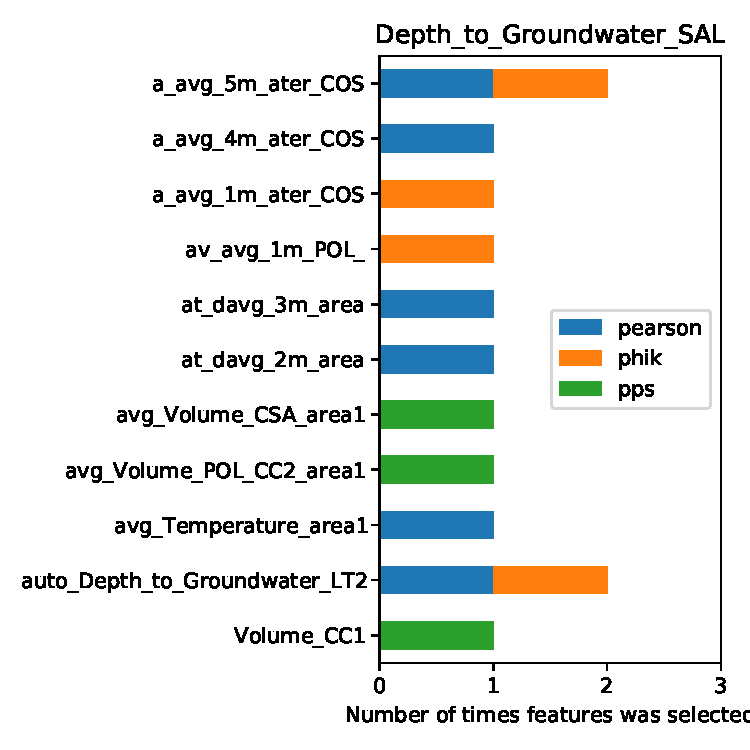
\includegraphics[width=0.45\textwidth]{figs/feature_selection_summary_Aquifer_Auser_Depth_to_Groundwater_SAL.pdf}
     \end{subfigure}
\caption{Features selection correlation/PPS-matrix for Aquifer Auser (target Depth to Groundwater SAL) using (top-left) $ \mathrm{abs}(\rho_p) > 0.4$, (top-right) $\phi_k > 0.8$ and (bottom-left) $PPS > 0.5$ for a prediction horizon on 60 days. The first row is the target variable. The selected features are strongly correlated amongst themselves. Note that the Pearson correlation ranges from $-1$ to $1$, indicating both the direction and the strength of the correlation, whereas the $\phi_k$ correlation ranges from $0$ to $1$ as it only describes the strength of the correlation. While for this target the overlap between the different feature selection methods is limited to two features (bottom-right).}
\label{fig:corr_auser}
\end{figure}

\subsection*{Implementation}

The common model interface of Sklearn's models allows for easy exploration of several regression models. Features and target are scaled to the range $[0, 1]$ in order to guarantee that all variables are of the same order of magnitude. This is of essential importance to some of the explored models, e.g. for neural network, as features at scales which differ in order of magnitude can lead to exploding weights. In addition tot the base model, six different regression  models will be explored: LinearModelRegression, MLPRegressor, SVR, RandomForestRegressor, GradientBoostingRegressor, GaussianProcessRegressor. 

In total 432 different models will be trained
\begin{itemize}
\item 8 targets which each have an unique set of selected features
\item 3 sets of selected features based on the 3 discussed feature selection methods 
\item 3 different prediction horizons: 7, 30 and 60 days
\item 6 different types of regression models
\end{itemize}

Cross validation is applied to study how well the model generalizes and get an estimate of the range of expected errors. The training period is chosen as two years and the test period 30 days. The time between the training period and test period is defined by the prediction horizon. The number of folds depends on the size of the respective datasets and varies between 20 and 150 folds.

Model selection and feature selection method is done simultaneously.  The selection based on the average performance of the model across the folds using the metrics $R^2$, $RMSE$, $MAE$ and $MAPE$. Model selection is carried out for each of the different feature selection methods. The best performing model across all different features selection methods and all the different models is selected and stored together with the selected feature selection method.

Hyper parameter tuning is carried out using Sklearn's GridSearch Class, using the cross validation schema defined in Fig.~\ref{fig:kfolds_cv}. 

% feature importance


\subsection*{Refinement}

The several refinement steps that have been taken evolve around
\begin{itemize}
\item Feature engineering, e.g. creation of an average Temperature or Rain features based on the different geographically located weather stations, or the creation of lagged features which are averaged over one month time.
\item Feature selection, e.g. the implementation of different feature selection methods and the study of the different selections on the model performance
\item Prediction horizon, as in the problem statement a priori no prediction horizon was defined, the possibilities for the usage of an ML model for different prediction horizons was explored
\item The training period, e.g different training periods have been explored. Short training periods insufficiently capture seasonal patterns whereas for longer periods too much information from old, irrelevant, data is included
\end{itemize}

More information about the above mentioned items can be found elsewhere in this document.

\FloatBarrier


\section{Results}

\subsection*{Model Evaluation and Validation}

The model performance is measured using the metrics $R^2$, $RMSE$, $MAE$ and $MAPE$. Cross validation is used to assess the generalisation of the models. 

The best prediction horizon was not a priori set. Different prediction horizons have been explored. As the target typically changes slowly over time it is not surprising that for short prediction horizons the base model performs best. Although the complex model perform similar to the base model in some cases, their behaviour is far less stable, as illustrated for Aquifer Auser, target Depth to Groundwater COS in Fig.~\ref{fig:auser_7d}. A similar behaviour -- and worse -- is observed for the other target variables. For a short prediction horizon the base model is therefore preferred. As no significant improvement over the base model is expected, no best ML is selected.

For a long prediction horizon of 60 days or longer, the additional regressors do contain information which allow the complex models to create a better prediction compared to the base model. After selection of the best set of features and the best model, cross validation is used for hyperparameter tuning. The optimal settings are listed in Tabs.~\ref{tab:gb_optim}-\ref{tab:svm_optim}. A list of selected features is included in Appendix A. Although the model performance is significantly better for some target values, it increases only slightly for others. An examples of an significantly increased model performance is illustrated in Fig.~\ref{fig:auser_cos_models} for Aquifer Auser Depth to Groundwater COS, while an example of a ML model with similar performance metrics to the base model can be found in Fig.~\ref{fig:arno_models} for River Arno Hydrometry Nave di Rosano. A complete overview of the best performing model per target can be found in Tab.~\ref{tab:bestm60}.


\begin{figure}
     \centering
     \begin{subfigure}
         \centering
         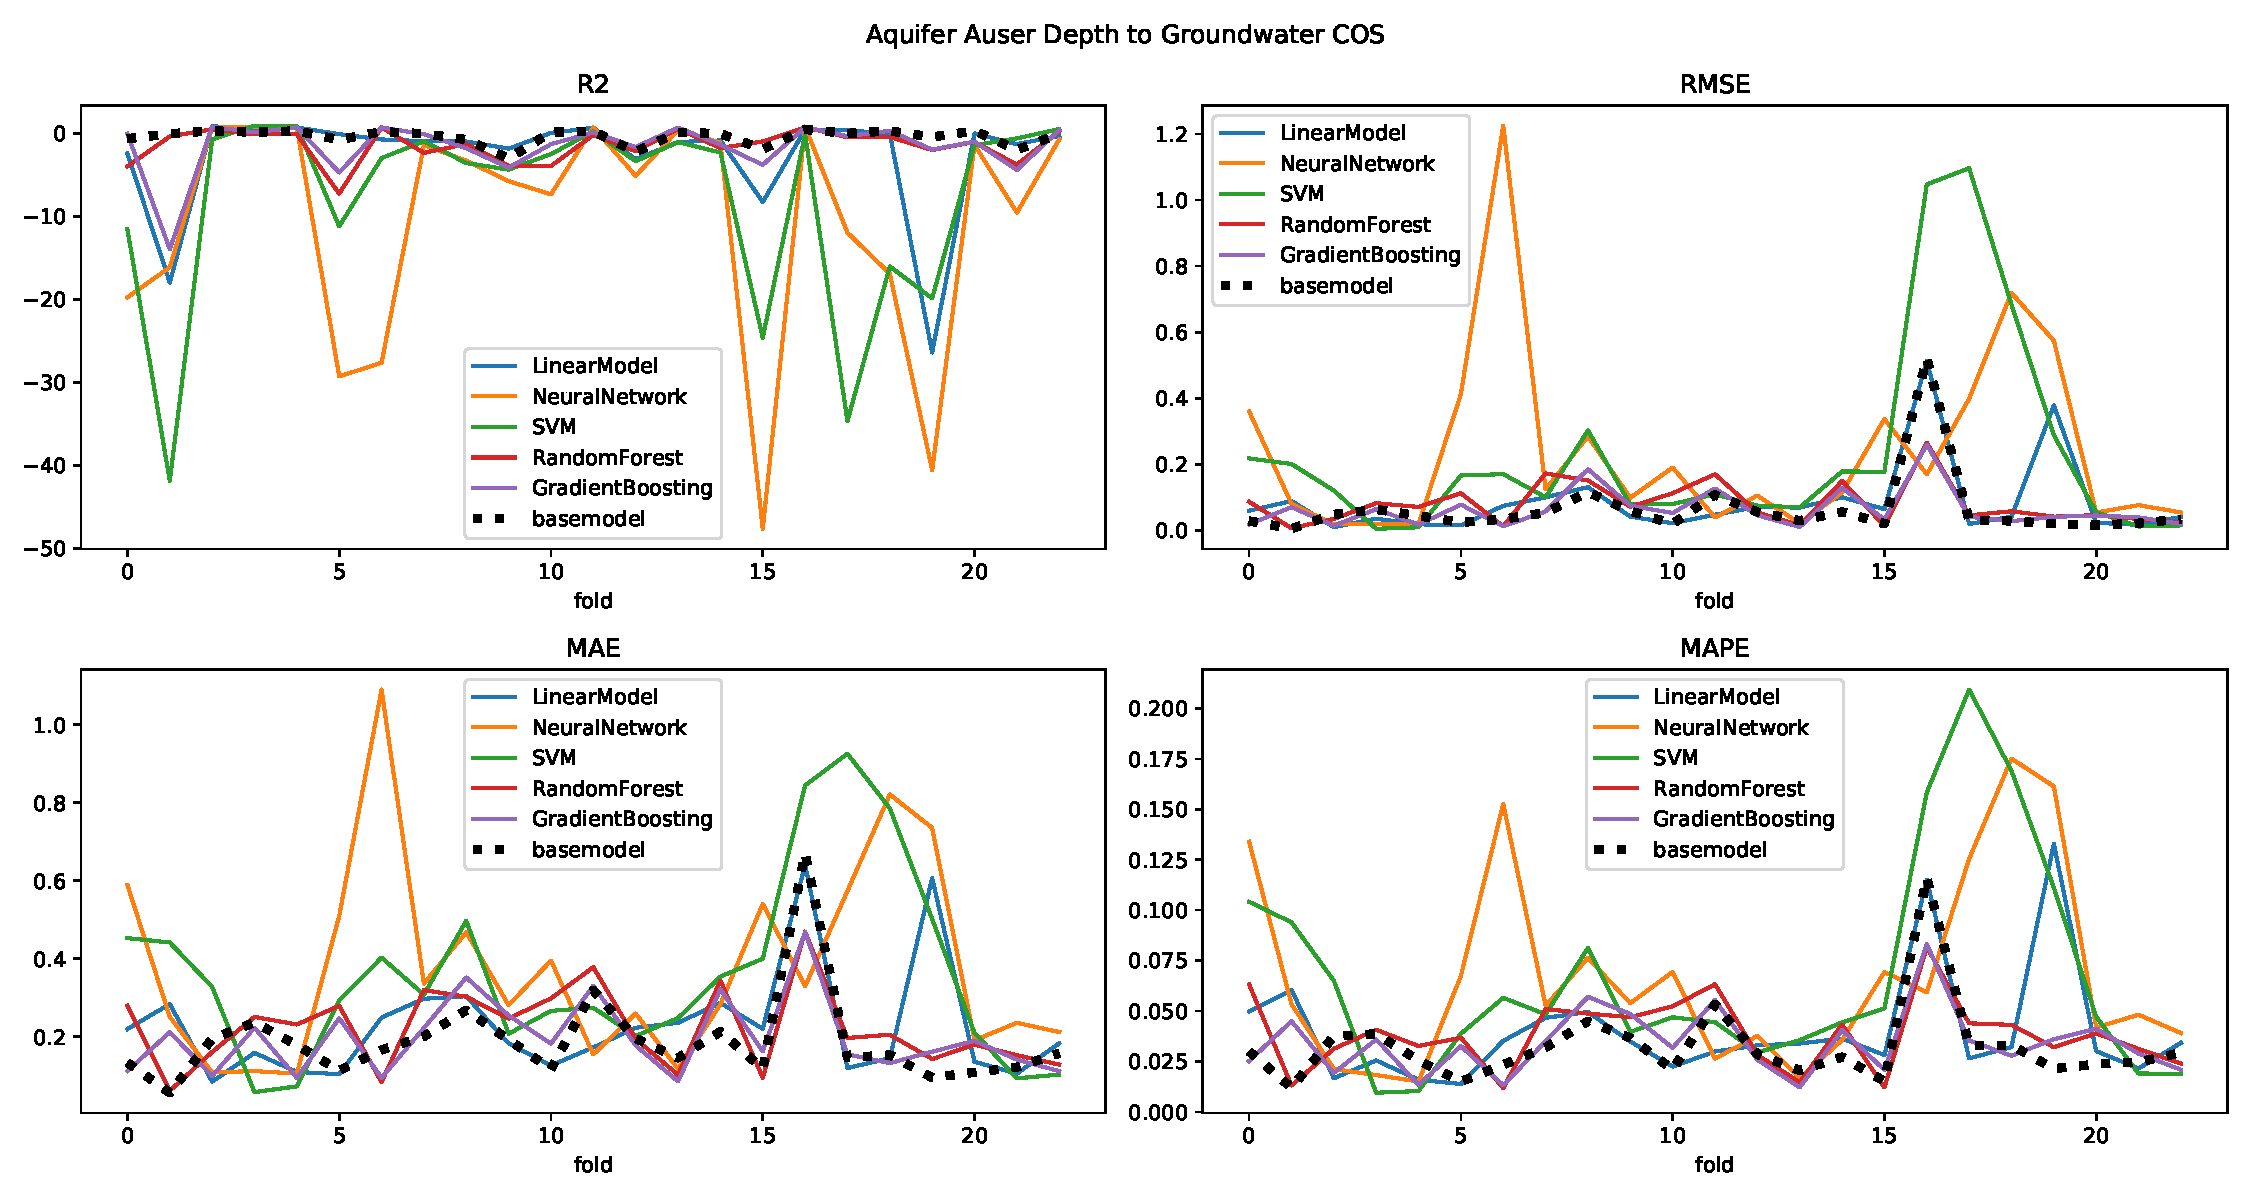
\includegraphics[width=0.9\textwidth]{figs/D7_pearson_Aquifer_Auser_Depth_to_Groundwater_COS_folds.pdf}
     \end{subfigure}
% 
     \begin{subfigure}
         \centering
         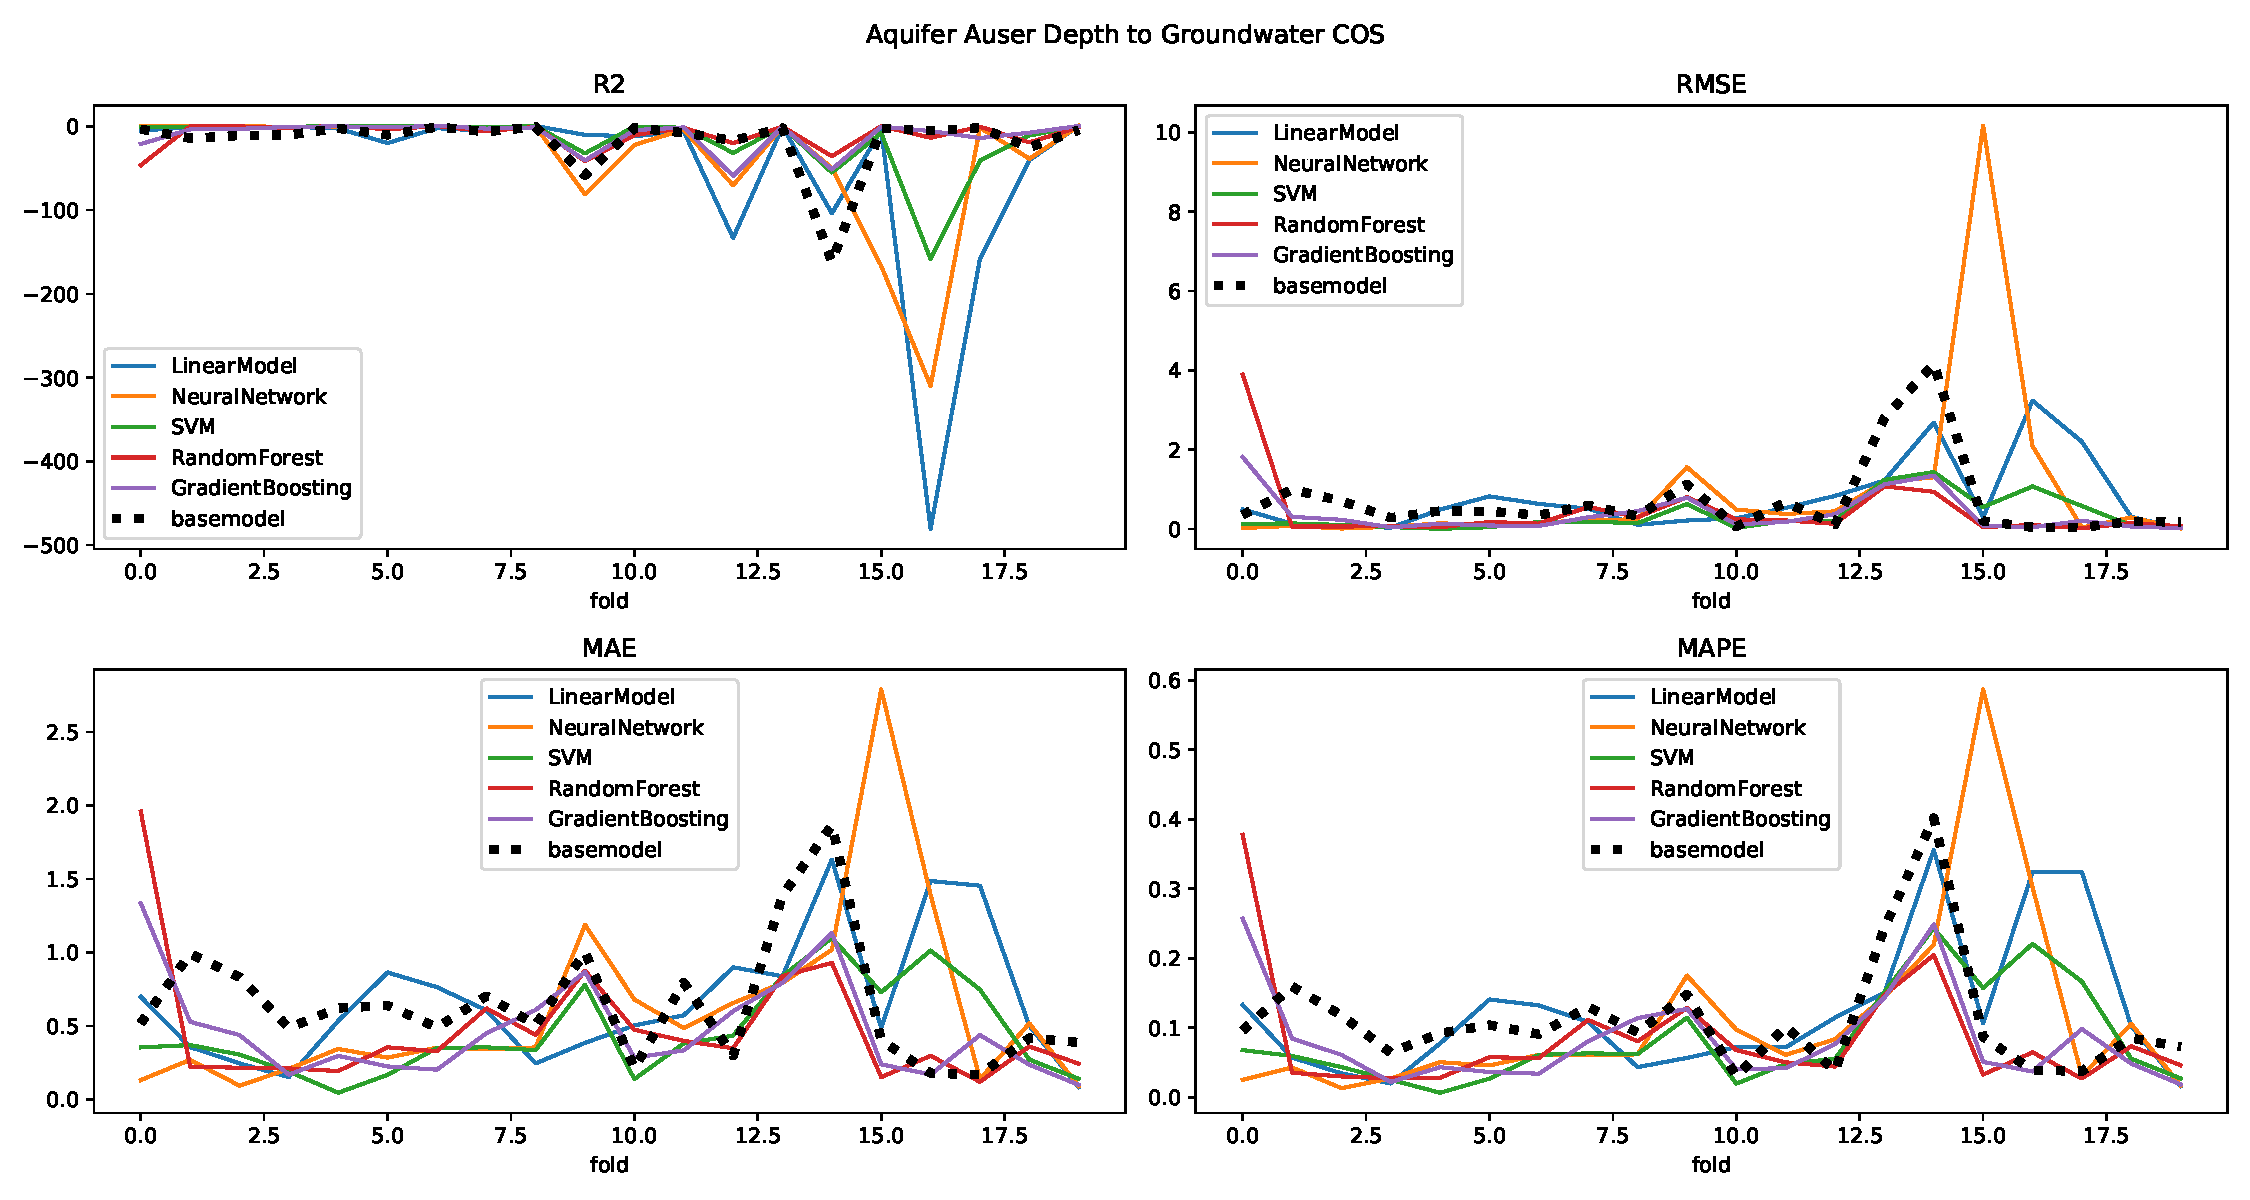
\includegraphics[width=0.9\textwidth]{figs/D30_pearson_Aquifer_Auser_Depth_to_Groundwater_COS_folds.pdf}
     \end{subfigure}

\caption{The model performance metrics $R^2$, RMSE, MAE and MAPE of the machine learning models (coloured lines) are compared to the base model (black dashed line). The base model outperforms the ML models for a 7-day and even a 30-day prediction horizon.}
\label{fig:auser_7d}
\end{figure}





\begin{table}[p]
\centering
\resizebox{0.9\textwidth}{!}{%
\begin{tabular}{lllrrl}
\toprule
     Water body &                    Target & Features &  learning\_rate &  n\_estimators &   loss \\
\midrule
  Aquifer Auser &  Depth to Groundwater COS &  pearson &           0.10 &           300 &  huber \\
 Lake Bilancino &                 Flow Rate &  pearson &           0.05 &           100 &    lad \\
\bottomrule
\end{tabular}
}
\caption{Features selection method and optimal model parameter for GradientBoosting. Hyper parameter not mentioned in this table are not considered during hyper parameter tuning.}
\label{tab:gb_optim}
\end{table}


\begin{table}[p]
\centering
\resizebox{0.7\textwidth}{!}{%
\begin{tabular}{lllrl}
\toprule
         Water body &                     Target & Features &     C &  kernel \\
\midrule
      Aquifer Auser &   Depth to Groundwater SAL &     phik &   1.0 &     rbf \\
 Aquifer Petrignano &   Depth to Groundwater P24 &     phik &   0.1 &     rbf \\
 Aquifer Petrignano &   Depth to Groundwater P25 &     phik &   1.0 &     rbf \\
     Lake Bilancino &                 Lake Level &     phik &   1.0 &     rbf \\
         River Arno &  Hydrometry Nave di Rosano &   manual &  10.0 &  linear \\
\bottomrule
\end{tabular}
}
\caption{Features selection method and optimal model parameter for SVM algorithm. Hyper parameter not mentioned in this table are not considered during hyper parameter tuning.}
\label{tab:svm_optim}
\end{table}


\begin{table}[p]
\centering
\resizebox{\textwidth}{!}{%
\begin{tabular}{lllllllrr}
\toprule
    Water body &                    Target & Features & solver &  hidden\_layer\_sizes &  early\_stopping &  max\_iter &  learning\_rate\_init \\
\midrule
 Aquifer Auser &  Depth to Groundwater LT2 &     phik &    sgd &              (200, 100) &            True &       800 &               0.001 \\
\bottomrule
\end{tabular}
}
\caption{Features selection method and optimal model parameter for Neural Network. Hyper parameter not mentioned in this table are not considered during hyper parameter tuning.}
\label{tab:nn_optim}
\end{table}

\begin{table}[htb]
\resizebox{\textwidth}{!}{%
\begin{tabular}{lllll}
\toprule
{} &                       r2 &                 rmse &                mae &               mape \\
\midrule
Aquifer\_Auser\_Depth\_to\_Groundwater\_COS      &       $ -4.01 \pm 6.39 $ &    $ 0.28 \pm 0.50 $ &  $ 0.38 \pm 0.31 $ &  $ 0.07 \pm 0.07 $ \\
Aquifer\_Auser\_Depth\_to\_Groundwater\_LT2      &       $ -6.08 \pm 5.19 $ &    $ 0.03 \pm 0.02 $ &  $ 0.14 \pm 0.08 $ &  $ 0.01 \pm 0.01 $ \\
Aquifer\_Auser\_Depth\_to\_Groundwater\_SAL      &     $ -11.46 \pm 24.06 $ &    $ 0.11 \pm 0.22 $ &  $ 0.24 \pm 0.19 $ &  $ 0.05 \pm 0.05 $ \\
Aquifer\_Petrignano\_Depth\_to\_Groundwater\_P24 &      $ -9.59 \pm 12.50 $ &    $ 0.42 \pm 0.38 $ &  $ 0.54 \pm 0.27 $ &  $ 0.02 \pm 0.01 $ \\
Aquifer\_Petrignano\_Depth\_to\_Groundwater\_P25 &     $ -11.06 \pm 12.14 $ &    $ 0.25 \pm 0.23 $ &  $ 0.41 \pm 0.22 $ &  $ 0.02 \pm 0.01 $ \\
Lake\_Bilancino\_Flow\_Rate                    &         $ -inf \pm inf $ &  $ 14.90 \pm 35.24 $ &  $ 1.77 \pm 2.46 $ &  $ 0.78 \pm 1.20 $ \\
Lake\_Bilancino\_Lake\_Level                   &  $ -260.96 \pm 1063.67 $ &    $ 0.92 \pm 1.08 $ &  $ 0.74 \pm 0.44 $ &  $ 0.00 \pm 0.00 $ \\
River\_Arno\_Hydrometry\_Nave\_di\_Rosano        &    $ -42.42 \pm 103.24 $ &    $ 0.32 \pm 0.43 $ &  $ 0.40 \pm 0.21 $ &  $ 0.26 \pm 0.11 $ \\
\bottomrule
\end{tabular}
}
\caption{Model evaluation metrics for the best model with a prediction horizon of 60 days. A comparison to the base model metrics in Tab.~\ref{tab:bm60} shows that, even though the model performance is still not great (negative r2), the best model performs better than the base model for all targets.}
\label{tab:bestm60}
\end{table}

\begin{figure}
     \centering
     \begin{subfigure}
         \centering
         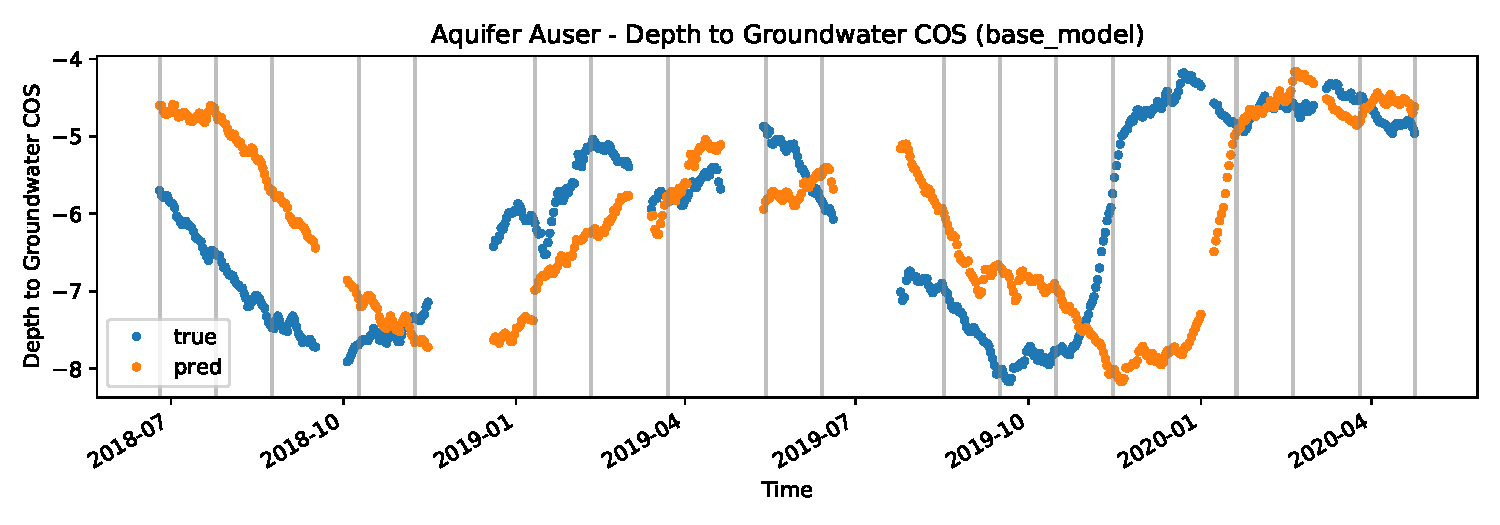
\includegraphics[width=0.9\textwidth]{figs/Aquifer_Auser_Depth_to_Groundwater_COS_base_model.pdf}
     \end{subfigure}
% 
     \begin{subfigure}
         \centering
         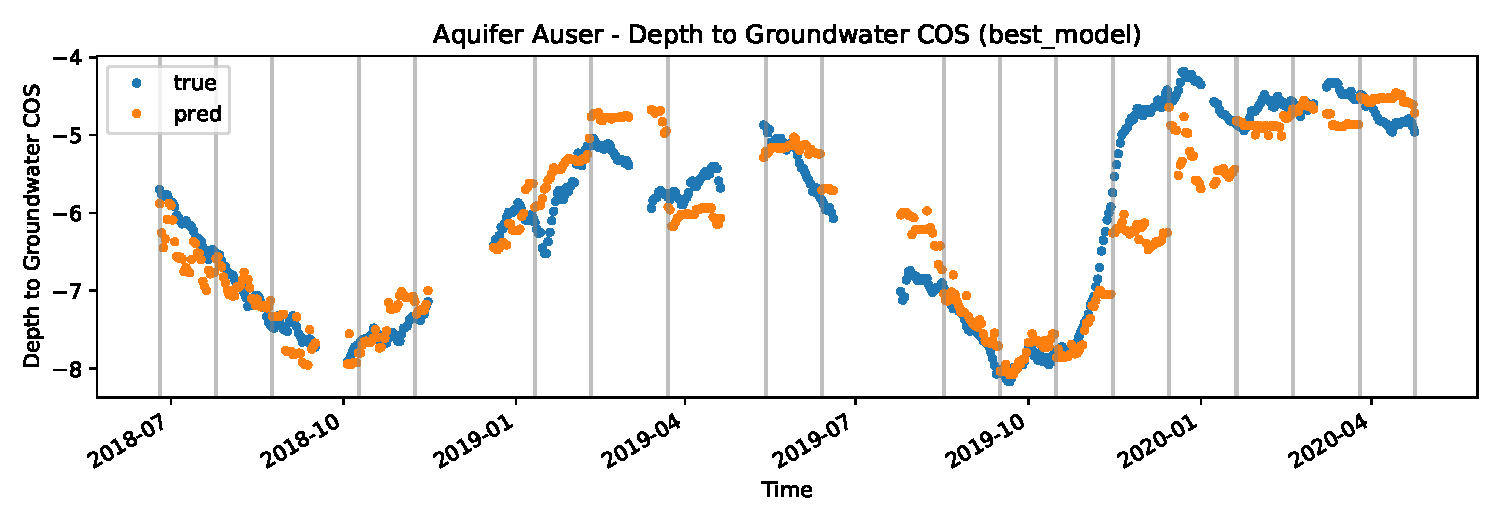
\includegraphics[width=0.9\textwidth]{figs/Aquifer_Auser_Depth_to_Groundwater_COS_best_model.pdf}
     \end{subfigure}
%
     \begin{subfigure}
         \centering
         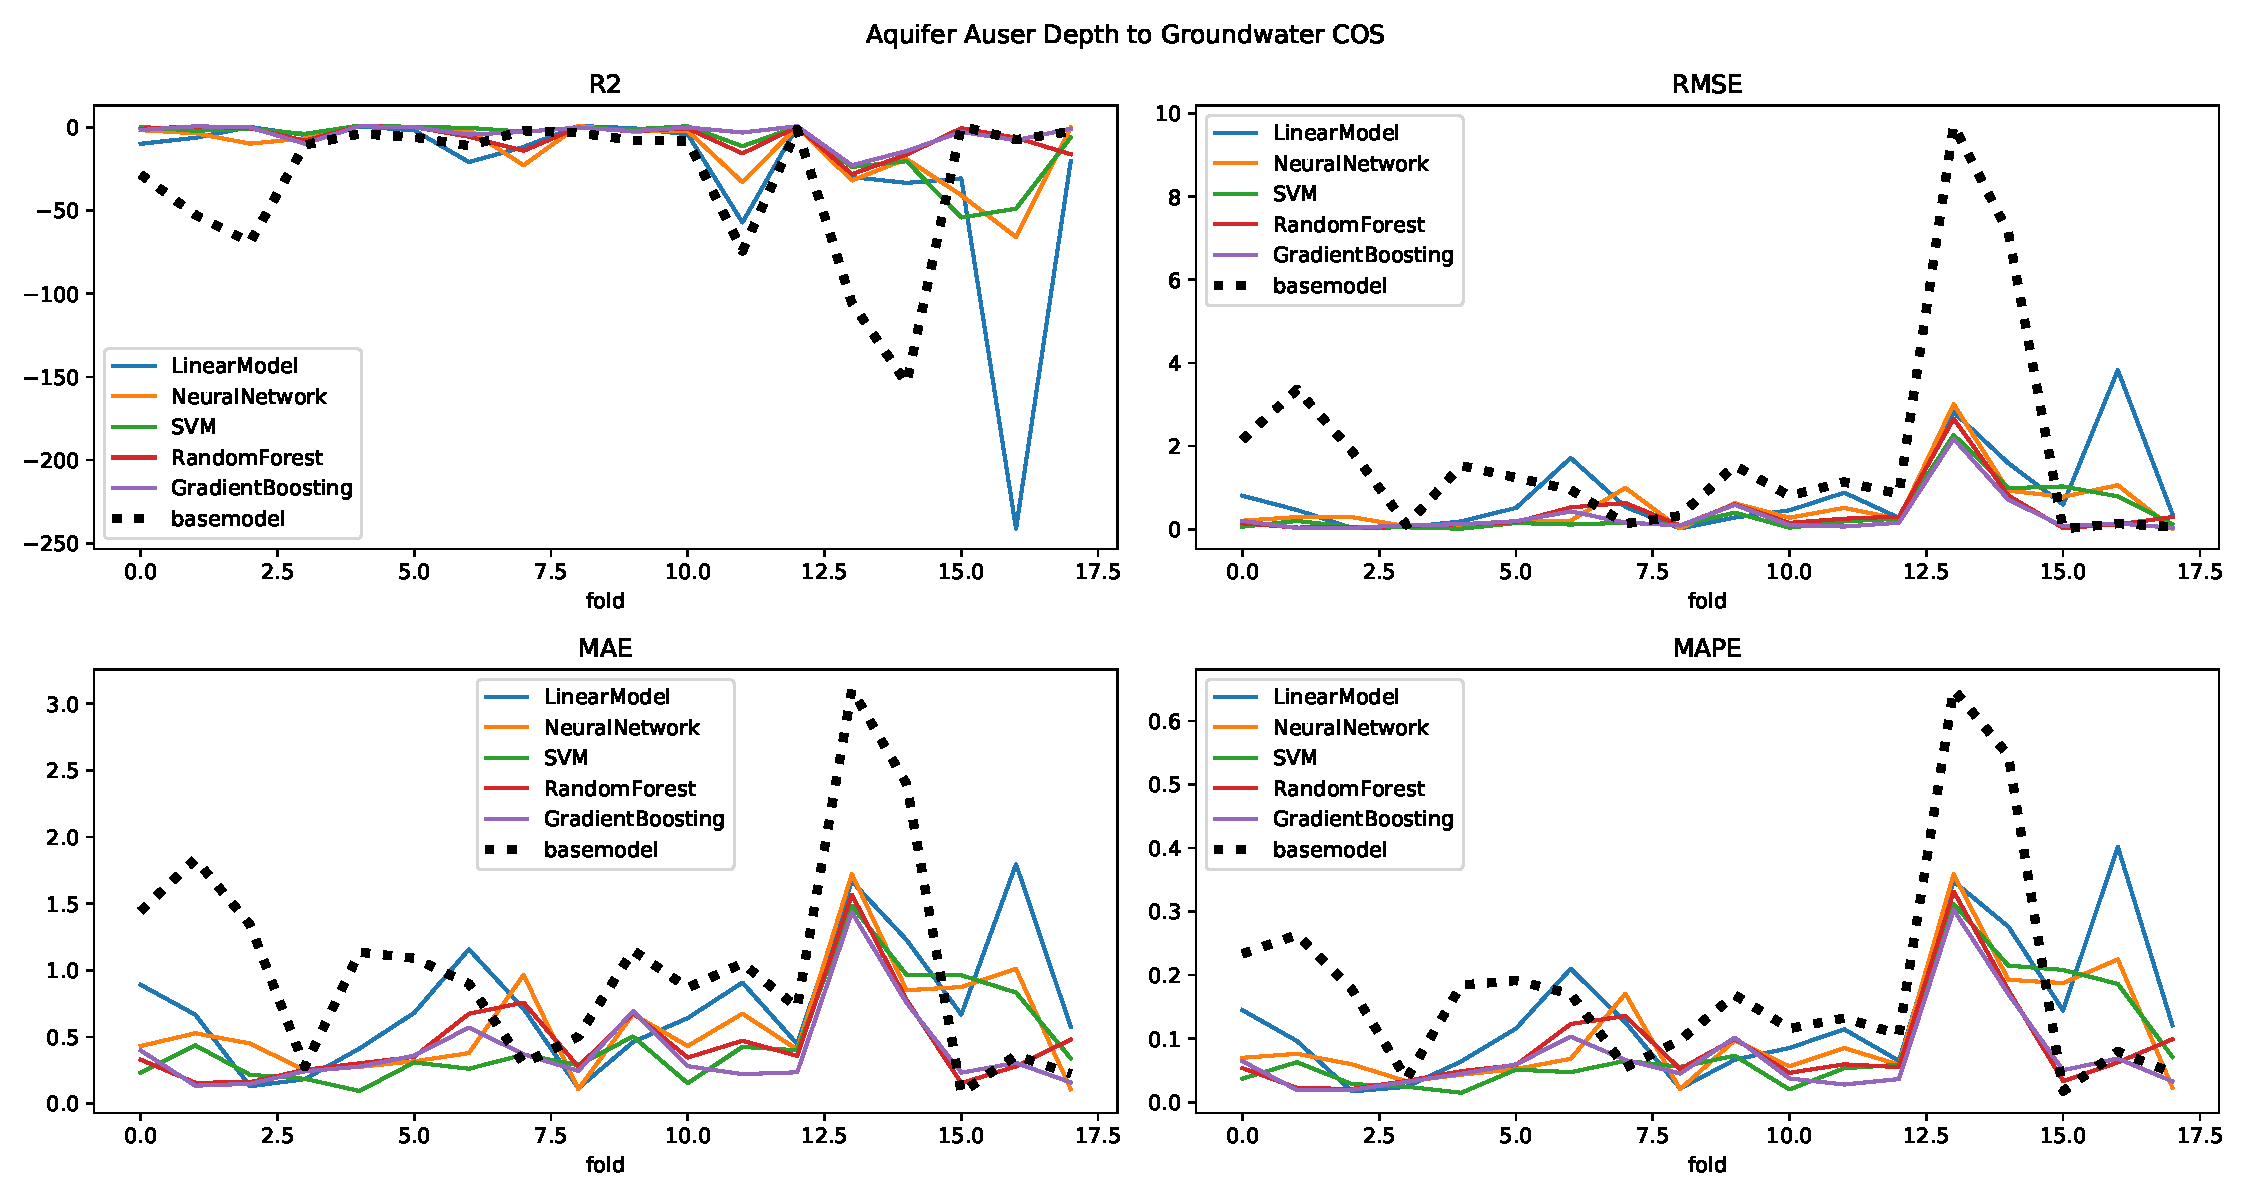
\includegraphics[width=0.9\textwidth]{figs/D60_pearson_Aquifer_Auser_Depth_to_Groundwater_COS_folds.pdf}
     \end{subfigure}
\caption{Model performance for Aquifer Auser, Depth to Groundwater COS, with a prediction horizon of 60 days. The best model (middle) better captures fluctuations in the ground water level than the base model (top). Different models have been evaluated (bottom) using cross validation. The model performance metrics $R^2$, RMSE, MAE and MAPE of the machine learning models (coloured lines) are compared to the base model (black dashed line). The different folds are indicated by the vertical grey lines in the top and middle plot. The best model has been reselected based on the mean RMSE over all the folds.}
\label{fig:auser_cos_models}
\end{figure}

\begin{figure}
     \centering
     \begin{subfigure}
         \centering
         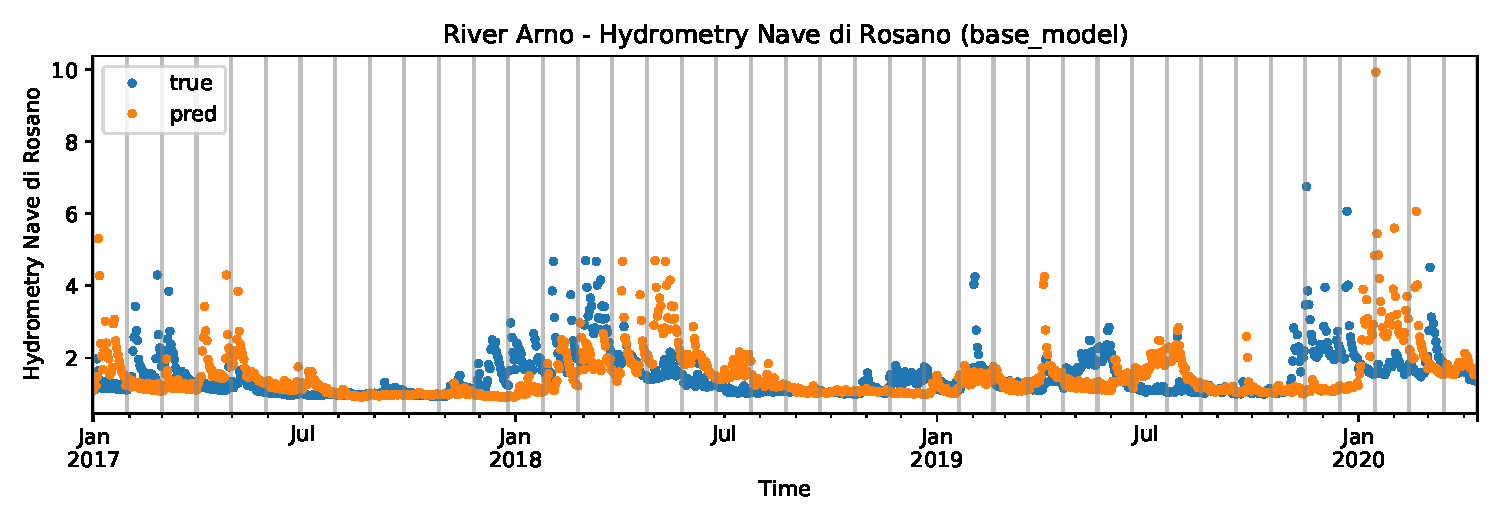
\includegraphics[width=0.9\textwidth]{figs/River_Arno_Hydrometry_Nave_di_Rosano_base_model.pdf}
     \end{subfigure}
% 
     \begin{subfigure}
         \centering
         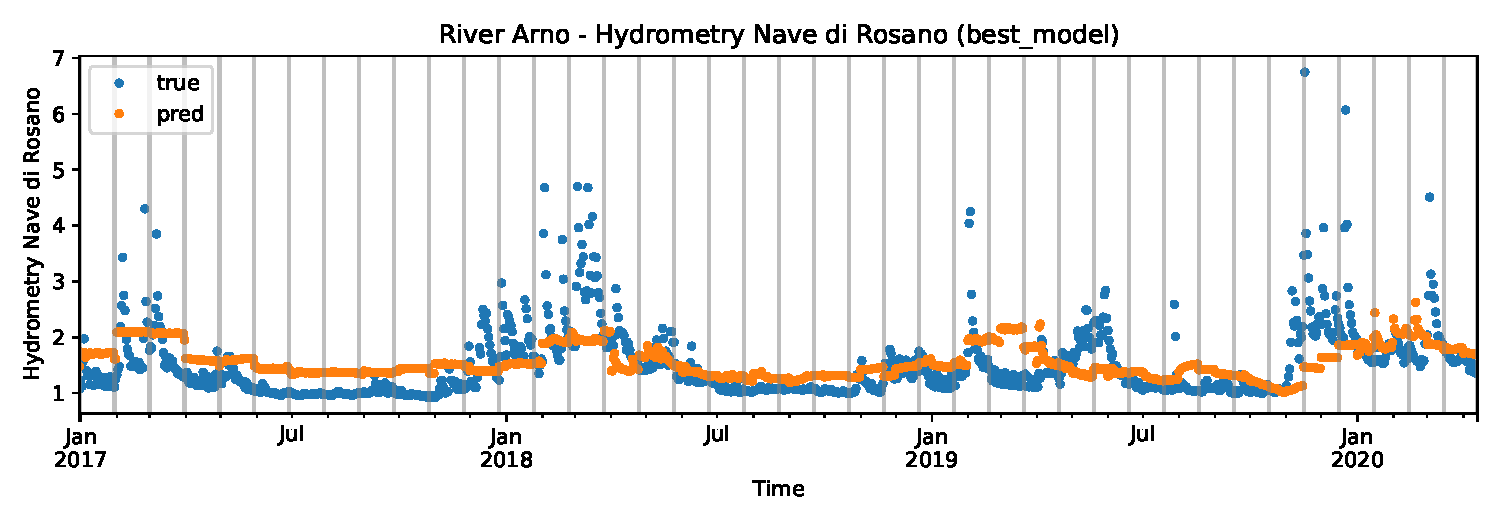
\includegraphics[width=0.9\textwidth]{figs/River_Arno_Hydrometry_Nave_di_Rosano_best_model.pdf}
     \end{subfigure}
%
     \begin{subfigure}
         \centering
         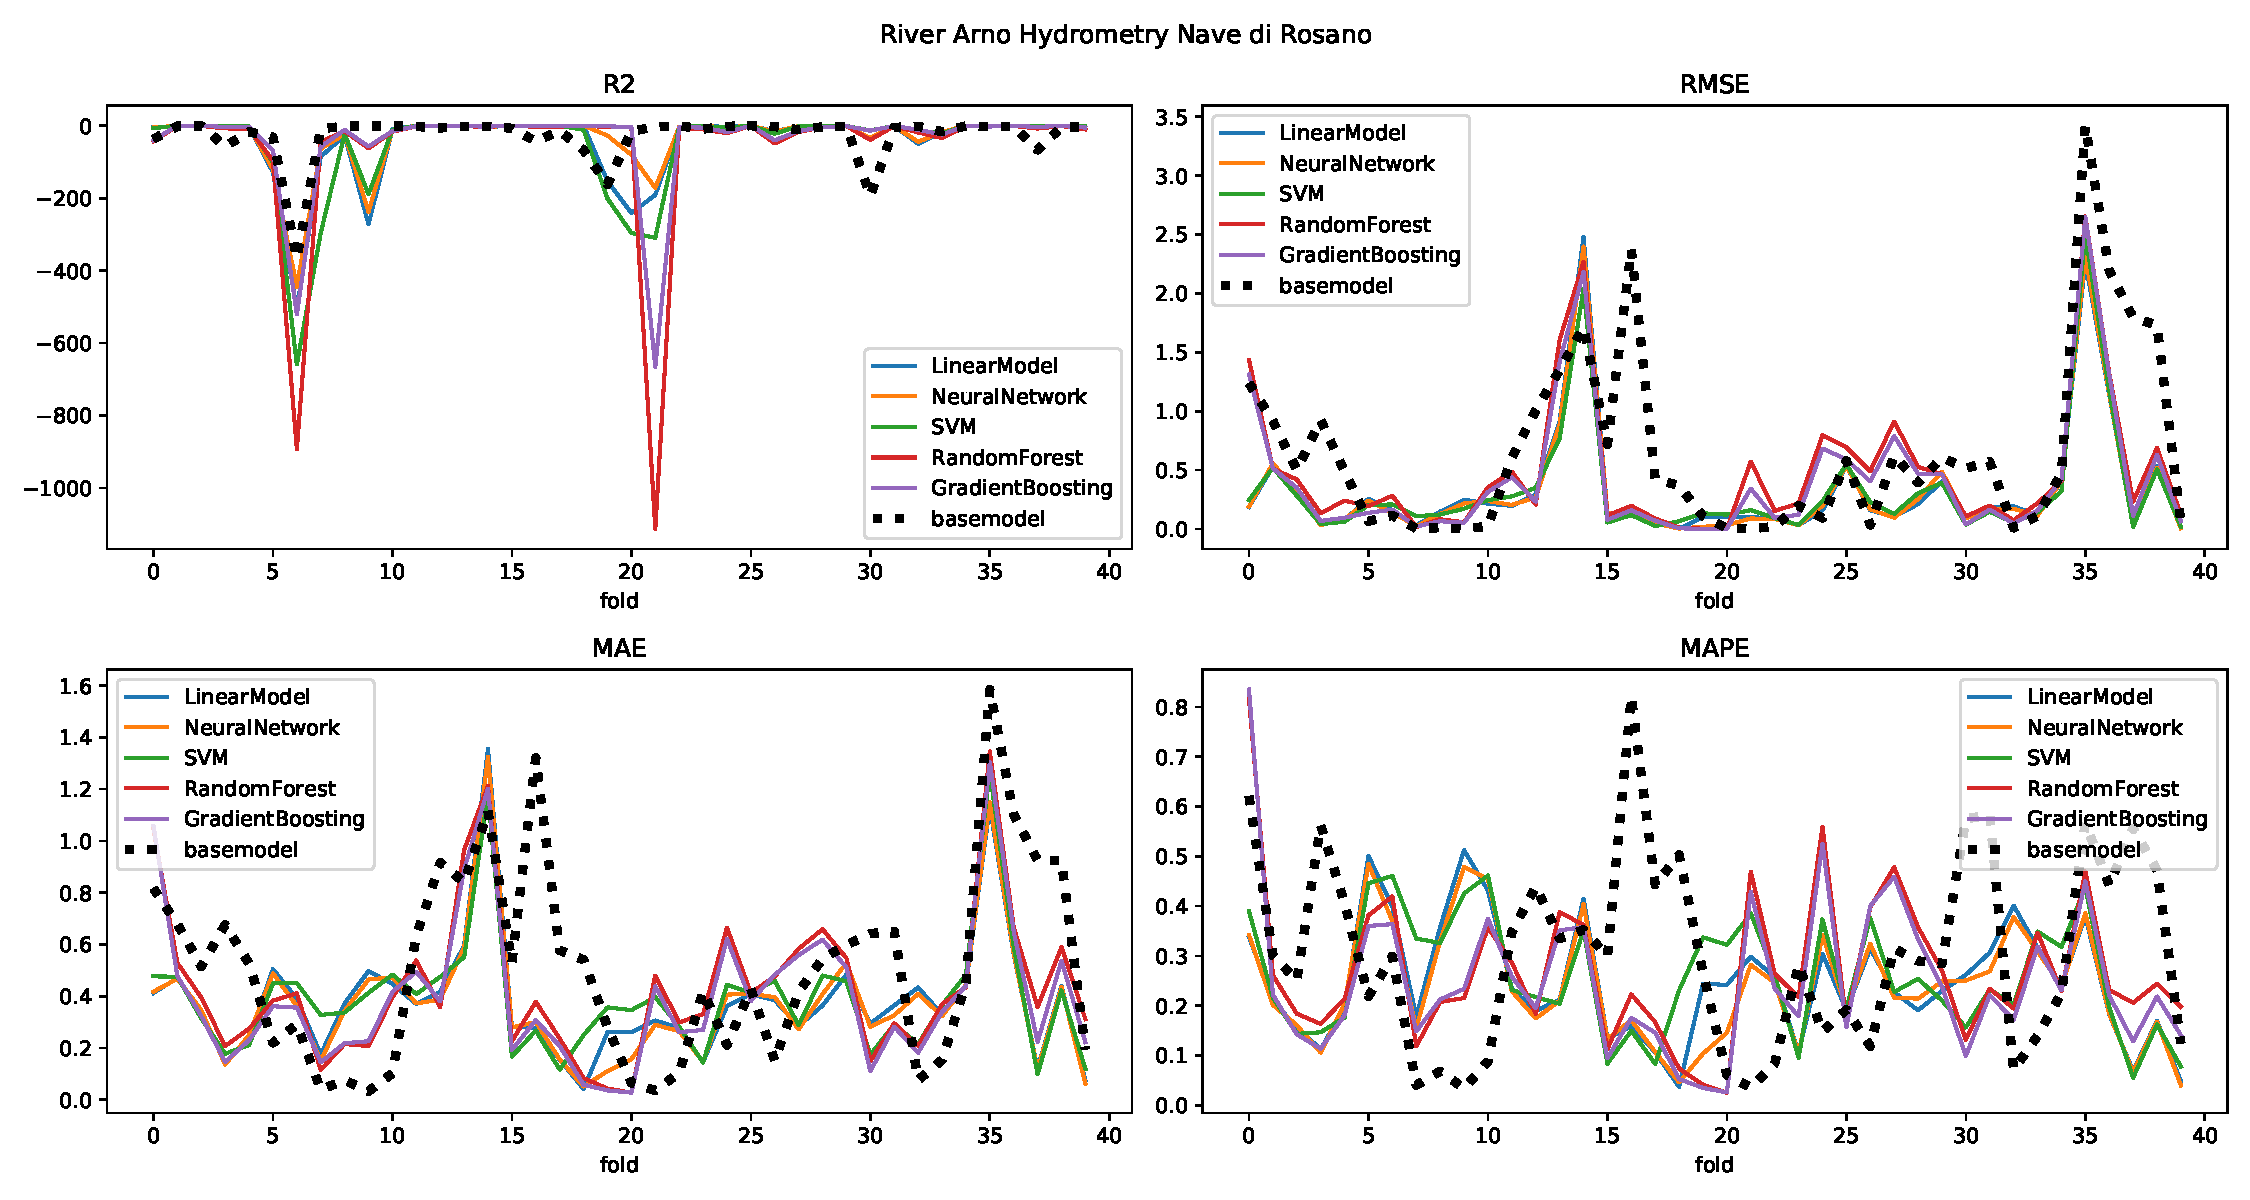
\includegraphics[width=0.9\textwidth]{figs/D60_pearson_River_Arno_Hydrometry_Nave_di_Rosano_folds.pdf}
     \end{subfigure}
\caption{Model performance for River Arno, Hydrometry Nave di Rosano, with a prediction horizon of 60 days. Although the best model (middle) performs slightly better in terms of RMSE than the base model (top), clearly all ML models fail to accurately capture variations in the river water level (bottom). The different ML models have been evaluation using cross validation. The different folds are indicated by the vertical grey lines in the top and middle plot. }
\label{fig:arno_models}
\end{figure}


\subsection*{Justification}

For a long prediction horizon of 60 days or longer, a ML model has an increased performance compared to the base model. For some target variables a consistent increase of model performance is observed over most cross validation folds and also between the different models. However, the uncertainty on the model evaluation is large, resulting in model performance metrics which are not significantly better. For other target variables the increase of model performance is marginal and clearly not significant. 

\FloatBarrier

\section{Conclusion}

The Acea Water group utilises nine different water bodies of varying types. In order to preserve the health of the water bodies and preserve continues water supply, Acea carefully monitors the water level in the different water bodies. Acea wishes to forecast the water level of its water bodies. Different prediction horizons have been explored. For a short prediction horizon, ranging from 1 week to 1 month, the use of an advanced ML model over a base model which simply uses the last known value as the prediction is not justified. For longer prediction horizons, starting from approximately six days, it has been observed that using a ML model slightly improves the forecast. Although model performance visually improves, the measured model performance metrics do not show a significant improvement. The increase of the model performance is strongly dependent on the (type of) target variable, as for some targets there is a clearly visible improvement while for others the ML model visually performs similar to the base model.

It is also noted that water level changes are not only an effect of environmental influences but are also steered by human interventions. When predicting with a 2 month prediction horizon, it is unlikely to think that one of the currently provided features is a good predictor of the human intervention that might occur in the next months. It could therefore be beneficial if some feature reflecting any planned interventions or processes can be included. 

It was also noted that it is up to the Acea Group to decide which water body to supply water from when water is used by the inhabitants of Italy. This leads to an interdependence of the different water bodies: water taken for use from one water body, does not need to be taken from another. It could therefore be beneficial to model the entire system of different water bodies at once.


\subsection*{Improvement}

Although further refinement of the feature engineering and feature selection procedures are possible, it is not expected to find a significant improvement of any of the current models. Given the nature of the data, a next step would be to explore the usage of models tuned to time series, such as Prophet~\cite{prophet} or Timeseers~\cite{timeseers}. These models allow for the inclusion of seasonal patterns, trends, trend-breaks and additional regressors. It is not unlikely that using these algorithms a better model than the current best model can be created. 

\subsection*{Reflection}

The entire process as carried out be best illustrated by a diagram, see Fig.~\ref{fig:process}. The difficulty of the project evolves around the multitude of different models that need to be trained. As the data included 9 different water bodies that each have multiple target variables, one could argue that this project was in fact 9 projects. Even though the same structure and analysis could be used for each water body or target, having to deal with so many different water bodies require a code structure to allow to quickly iterate and re-use code. 

\begin{figure}[htb]
\begin{center}
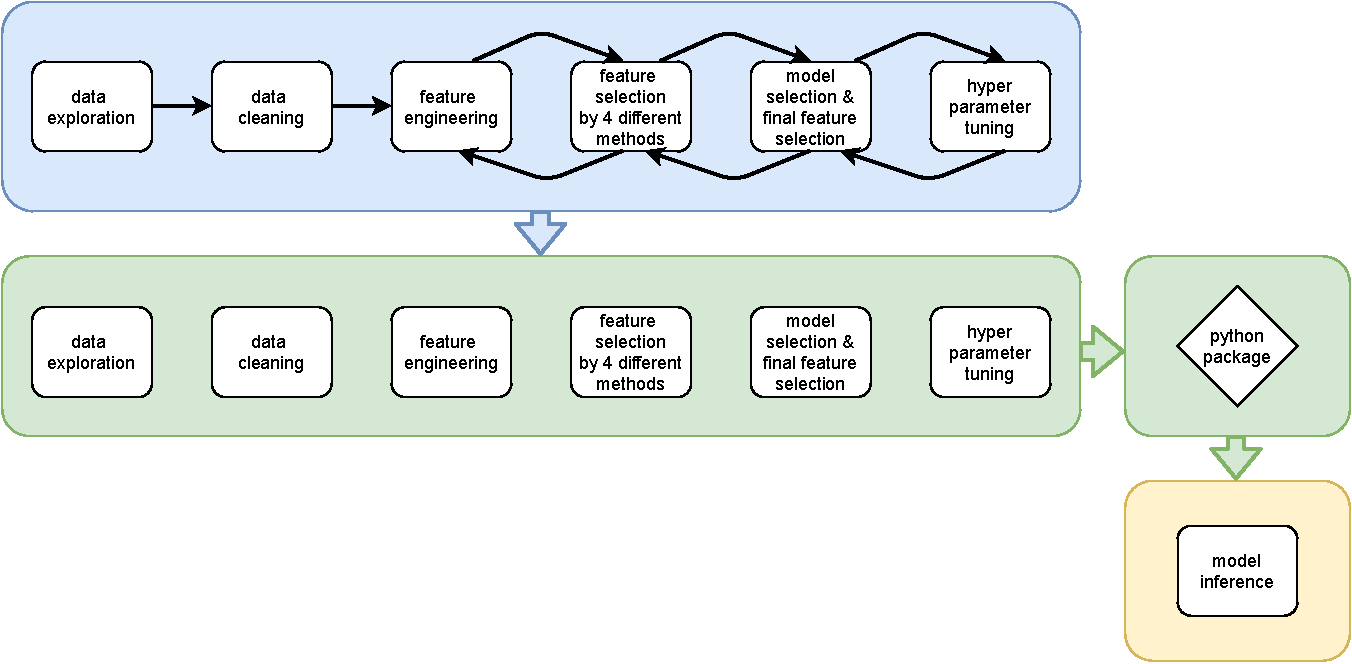
\includegraphics[width=0.9\textwidth]{figs/project_process.pdf}
\caption{The different steps taken in the Acea Water project. The blue bar indicates the iterative process one goes through to when developing a model. Once all process steps have been defined and a draft pipeline has been achieved, the relevant, repeatable, components are moved to a python package, indicated with the green bar. The functionality from the python package can then be used by the inference code, indicated in yellow. All the preprocessing and feature engineering steps are now taken from the python package to guarantee exactly the same steps are taken in model training and model inference.}
\label{fig:process}
\end{center}
\end{figure}


\FloatBarrier

\newpage

\section*{Appendix A}

An overview of the features selected for the best models is included in Tabs.~\ref{tab:feats1}-\ref{tab:feats3}.

Feature names explained:

\begin{itemize}
\item prefix = avg: average of several features of the same type, for instance several Temperature features
\item prefix = auto: auto correlation of the target. This is the value of the target at t = t0 - prediction horizon
\item prefix = t: temperature
\item prefix = r: rainfall
\item prefix = d: depth of groundwater
\item prefix = v: volume
\item prefix = h: hydrometry
\item prefix = t\_avg\_1m: the average temperature calculated over the previous month   
\item prefix = t\_avg\_2m: the average temperature calculated over the month before the previous month (same for 3m, 4m, 5m, 6m)
\item prefix = v\_avg\_xm or h\_avg\_xm or r\_avg\_xm or d\_avg\_xm: same as the above to items for volume, hydrometry, rainfall, depth of groundwater
\item prefix = at\_avg\_1m\_area1: the average temperature calculated over the previous month, measured by the average of several features that together span area1  
\item prefix = at\_avg\_2m\_area1: the average temperature calculated over the month before the previous month, measured by the average of several features that together span area1 (same for 3m, 4m, 5m, 6m) 
\item prefix = av\_avg\_xm or ah\_avg\_xm or ar\_avg\_xm or ad\_avg\_xm: same as the above to items for volume, hydrometry, rainfall, depth of groundwater
\end{itemize}


\begin{table}
\resizebox{0.9\textwidth}{!}{%
\begin{tabular}{lll}
\toprule
               Body &                     Target &                        Features \\
\midrule
      Aquifer Auser &   Depth\_to\_Groundwater\_COS &  avg\_Depth\_to\_Groundwater\_area1 \\
      Aquifer Auser &   Depth\_to\_Groundwater\_COS &        avg\_Volume\_POL\_CC2\_area1 \\
      Aquifer Auser &   Depth\_to\_Groundwater\_COS &   auto\_Depth\_to\_Groundwater\_COS \\
      Aquifer Auser &   Depth\_to\_Groundwater\_COS &            avg\_Volume\_CSA\_area1 \\
      Aquifer Auser &   Depth\_to\_Groundwater\_COS &   auto\_Depth\_to\_Groundwater\_SAL \\
      Aquifer Auser &   Depth\_to\_Groundwater\_COS &                  ah\_avg\_1m\_area \\
      Aquifer Auser &   Depth\_to\_Groundwater\_COS &                  av\_avg\_1m\_POL\_ \\
      Aquifer Auser &   Depth\_to\_Groundwater\_COS &                  av\_avg\_1m\_CSA\_ \\
      Aquifer Auser &   Depth\_to\_Groundwater\_COS &                 ad\_davg\_3m\_area \\
      Aquifer Auser &   Depth\_to\_Groundwater\_COS &               a\_avg\_1m\_ater\_SAL \\
      Aquifer Auser &   Depth\_to\_Groundwater\_COS &                  ad\_avg\_1m\_area \\
      Aquifer Auser &   Depth\_to\_Groundwater\_COS &            avg\_Hydrometry\_area1 \\
      Aquifer Auser &   Depth\_to\_Groundwater\_COS &                 ad\_davg\_2m\_area \\
      Aquifer Auser &   Depth\_to\_Groundwater\_COS &                         month\_9 \\
      Aquifer Auser &   Depth\_to\_Groundwater\_COS &                  at\_avg\_2m\_area \\
      Aquifer Auser &   Depth\_to\_Groundwater\_COS &                 at\_davg\_2m\_area \\
      Aquifer Auser &   Depth\_to\_Groundwater\_COS &               a\_avg\_4m\_ater\_COS \\
      Aquifer Auser &   Depth\_to\_Groundwater\_COS &               a\_avg\_6m\_ater\_COS \\
      Aquifer Auser &   Depth\_to\_Groundwater\_COS &               a\_avg\_5m\_ater\_COS \\
      Aquifer Auser &   Depth\_to\_Groundwater\_COS &                 at\_davg\_3m\_area \\
      Aquifer Auser &   Depth\_to\_Groundwater\_COS &                  at\_avg\_1m\_area \\
      Aquifer Auser &   Depth\_to\_Groundwater\_COS &           avg\_Temperature\_area1 \\
      Aquifer Auser &   Depth\_to\_Groundwater\_LT2 &                  ad\_avg\_2m\_area \\
      Aquifer Auser &   Depth\_to\_Groundwater\_LT2 &                    v\_avg\_3m\_CC1 \\
      Aquifer Auser &   Depth\_to\_Groundwater\_LT2 &                    v\_avg\_2m\_CC1 \\
      Aquifer Auser &   Depth\_to\_Groundwater\_LT2 &                  av\_avg\_2m\_POL\_ \\
      Aquifer Auser &   Depth\_to\_Groundwater\_LT2 &                 ad\_davg\_2m\_area \\
      Aquifer Auser &   Depth\_to\_Groundwater\_LT2 &                   v\_davg\_2m\_CC1 \\
      Aquifer Auser &   Depth\_to\_Groundwater\_LT2 &               a\_avg\_6m\_ater\_LT2 \\
      Aquifer Auser &   Depth\_to\_Groundwater\_LT2 &               a\_avg\_2m\_ater\_LT2 \\
      Aquifer Auser &   Depth\_to\_Groundwater\_LT2 &                 av\_davg\_2m\_POL\_ \\
      Aquifer Auser &   Depth\_to\_Groundwater\_LT2 &                  at\_avg\_3m\_area \\
      Aquifer Auser &   Depth\_to\_Groundwater\_LT2 &               a\_avg\_3m\_ater\_LT2 \\
      Aquifer Auser &   Depth\_to\_Groundwater\_LT2 &                  av\_avg\_2m\_CSA\_ \\
      Aquifer Auser &   Depth\_to\_Groundwater\_LT2 &                  at\_avg\_2m\_area \\
      Aquifer Auser &   Depth\_to\_Groundwater\_LT2 &               a\_avg\_2m\_ater\_COS \\
      Aquifer Auser &   Depth\_to\_Groundwater\_SAL &                  av\_avg\_1m\_POL\_ \\
      Aquifer Auser &   Depth\_to\_Groundwater\_SAL &   auto\_Depth\_to\_Groundwater\_LT2 \\
      Aquifer Auser &   Depth\_to\_Groundwater\_SAL &               a\_avg\_1m\_ater\_COS \\
      Aquifer Auser &   Depth\_to\_Groundwater\_SAL &               a\_avg\_5m\_ater\_COS \\

\bottomrule
\end{tabular}}
\caption{List of features in best model (prediction horizon 60 days)}
\label{tab:feats1}
\end{table}

\begin{table}
\resizebox{0.9\textwidth}{!}{%
\begin{tabular}{lll}
\toprule
               Body &                     Target &                        Features \\
\midrule
 Aquifer Petrignano &   Depth\_to\_Groundwater\_P24 &   auto\_Depth\_to\_Groundwater\_P25 \\
 Aquifer Petrignano &   Depth\_to\_Groundwater\_P24 &   auto\_Depth\_to\_Groundwater\_P24 \\
 Aquifer Petrignano &   Depth\_to\_Groundwater\_P24 &               a\_avg\_1m\_ater\_P24 \\
 Aquifer Petrignano &   Depth\_to\_Groundwater\_P24 &                  at\_avg\_3m\_area \\
 Aquifer Petrignano &   Depth\_to\_Groundwater\_P24 &               a\_avg\_1m\_ater\_P25 \\
 Aquifer Petrignano &   Depth\_to\_Groundwater\_P24 &                   h\_avg\_1m\_Fium \\
 Aquifer Petrignano &   Depth\_to\_Groundwater\_P24 &                   v\_avg\_1m\_C10\_ \\
 Aquifer Petrignano &   Depth\_to\_Groundwater\_P24 &               a\_avg\_6m\_ater\_P24 \\
 Aquifer Petrignano &   Depth\_to\_Groundwater\_P24 &               a\_avg\_6m\_ater\_P25 \\
 Aquifer Petrignano &   Depth\_to\_Groundwater\_P25 &   auto\_Depth\_to\_Groundwater\_P25 \\
 Aquifer Petrignano &   Depth\_to\_Groundwater\_P25 &   auto\_Depth\_to\_Groundwater\_P24 \\
 Aquifer Petrignano &   Depth\_to\_Groundwater\_P25 &               a\_avg\_1m\_ater\_P25 \\
 Aquifer Petrignano &   Depth\_to\_Groundwater\_P25 &               a\_avg\_1m\_ater\_P24 \\
 Aquifer Petrignano &   Depth\_to\_Groundwater\_P25 &                  at\_avg\_3m\_area \\
 Aquifer Petrignano &   Depth\_to\_Groundwater\_P25 &                   v\_avg\_1m\_C10\_ \\
 Aquifer Petrignano &   Depth\_to\_Groundwater\_P25 &                   h\_avg\_1m\_Fium \\
 Aquifer Petrignano &   Depth\_to\_Groundwater\_P25 &                  at\_avg\_2m\_area \\
 Aquifer Petrignano &   Depth\_to\_Groundwater\_P25 &                   v\_avg\_2m\_C10\_ \\
 Aquifer Petrignano &   Depth\_to\_Groundwater\_P25 &                   h\_avg\_3m\_Fium \\
 Aquifer Petrignano &   Depth\_to\_Groundwater\_P25 &                   v\_avg\_3m\_C10\_ \\
 Aquifer Petrignano &   Depth\_to\_Groundwater\_P25 &               a\_avg\_6m\_ater\_P24 \\
 Aquifer Petrignano &   Depth\_to\_Groundwater\_P25 &                 at\_davg\_2m\_area \\
 Aquifer Petrignano &   Depth\_to\_Groundwater\_P25 &               a\_avg\_6m\_ater\_P25 \\
     Lake Bilancino &                  Flow\_Rate &               a\_avg\_3m\_ke\_Level \\
     Lake Bilancino &                  Flow\_Rate &                 auto\_Lake\_Level \\
     Lake Bilancino &                  Flow\_Rate &              avg\_Rainfall\_area1 \\
     Lake Bilancino &                  Flow\_Rate &                         month\_1 \\
     Lake Bilancino &                  Flow\_Rate &                         month\_2 \\
     Lake Bilancino &                  Flow\_Rate &                         month\_3 \\
     Lake Bilancino &                  Flow\_Rate &                         month\_4 \\
     Lake Bilancino &                  Flow\_Rate &                         month\_5 \\
     Lake Bilancino &                  Flow\_Rate &                         month\_6 \\
     Lake Bilancino &                  Flow\_Rate &                         month\_7 \\
     Lake Bilancino &                  Flow\_Rate &                         month\_8 \\
     Lake Bilancino &                  Flow\_Rate &                         month\_9 \\
     Lake Bilancino &                  Flow\_Rate &                        month\_10 \\
     Lake Bilancino &                  Flow\_Rate &                        month\_11 \\
     Lake Bilancino &                  Flow\_Rate &                        month\_12 \\
     Lake Bilancino &                 Lake\_Level &                 auto\_Lake\_Level \\
     Lake Bilancino &                 Lake\_Level &               a\_avg\_1m\_low\_Rate \\
     Lake Bilancino &                 Lake\_Level &                         month\_1 \\
     Lake Bilancino &                 Lake\_Level &                         month\_2 \\
     Lake Bilancino &                 Lake\_Level &                         month\_3 \\
     Lake Bilancino &                 Lake\_Level &                         month\_4 \\
     Lake Bilancino &                 Lake\_Level &                         month\_5 \\
     Lake Bilancino &                 Lake\_Level &                         month\_6 \\
     Lake Bilancino &                 Lake\_Level &                         month\_7 \\
     Lake Bilancino &                 Lake\_Level &                         month\_8 \\
     Lake Bilancino &                 Lake\_Level &                         month\_9 \\
     Lake Bilancino &                 Lake\_Level &                        month\_10 \\
     Lake Bilancino &                 Lake\_Level &                        month\_11 \\
\bottomrule
\end{tabular}}
\caption{List of features in best model (prediction horizon 60 days), continued.}
\label{tab:feats2}
\end{table}




%
\begin{table}
\resizebox{0.9\textwidth}{!}{%
\begin{tabular}{lll}
\toprule
               Body &                     Target &                        Features \\
\midrule
         River Arno &  Hydrometry\_Nave\_di\_Rosano &               a\_avg\_4m\_i\_Rosano \\
         River Arno &  Hydrometry\_Nave\_di\_Rosano &  auto\_Hydrometry\_Nave\_di\_Rosano \\
         River Arno &  Hydrometry\_Nave\_di\_Rosano &                         month\_1 \\
         River Arno &  Hydrometry\_Nave\_di\_Rosano &                         month\_2 \\
         River Arno &  Hydrometry\_Nave\_di\_Rosano &                         month\_3 \\
         River Arno &  Hydrometry\_Nave\_di\_Rosano &                         month\_4 \\
         River Arno &  Hydrometry\_Nave\_di\_Rosano &                         month\_5 \\
         River Arno &  Hydrometry\_Nave\_di\_Rosano &                         month\_6 \\
         River Arno &  Hydrometry\_Nave\_di\_Rosano &                         month\_7 \\
         River Arno &  Hydrometry\_Nave\_di\_Rosano &                         month\_8 \\
         River Arno &  Hydrometry\_Nave\_di\_Rosano &                         month\_9 \\
         River Arno &  Hydrometry\_Nave\_di\_Rosano &                        month\_10 \\
         River Arno &  Hydrometry\_Nave\_di\_Rosano &                        month\_11 \\
         River Arno &  Hydrometry\_Nave\_di\_Rosano &                        month\_12 \\
\bottomrule
\end{tabular}}
\caption{List of features in best model (prediction horizon 60 days), continued.}
\label{tab:feats3}
\end{table}
%

\begin{thebibliography}{9}

\bibitem{acea} 
Acea Group \\\texttt{https://www.gruppo.acea.it/en}

\bibitem{kaggle} 
Kaggle competition Acea Smart Water Analytics \\\texttt{https://www.kaggle.com/c/acea-water-prediction}

\bibitem{pearson}
K. Pearson, \textit{Proceedings of the Royal Society of London} (1854-1905) 58, 240242 (1895).

\bibitem{phik}
M. Baak, R. Koopman, H. Snoek, S. Klous,
\textit{A new correlation coefficient between categorical, ordinal and interval variables with Pearson characteristics}
Computational Statistics \& Data Analysis,
Volume 152,
2020,
107043,
ISSN 0167-9473

\bibitem{pps}
Rip correlation. Introducing the predictive power score \\\texttt{https://8080labs.com/blog/posts/rip-correlation-introducing-the-predictive-power-score-pps/}

\bibitem{prophet}
Taylor SJ, Letham B. 2017. \textit{Forecasting at scale}. PeerJ Preprints 5:e3190v2

\bibitem{timeseers}
M. Brouns, Timeseers \\\texttt{https://github.com/MBrouns/timeseers}

\end{thebibliography}

\newpage


\end{document}